\documentclass[twoside,9pt]{report}
\usepackage[a5paper]{geometry}
\usepackage{newpxmath}
%\usepackage{libertine} \usepackage[libertine]{newtxmath}
%\usepackage{kpfonts}
\usepackage{graphicx}
\usepackage{listings}
\usepackage[T1]{fontenc}
\usepackage{imakeidx}
\lstset{
  showstringspaces=false,
  language=tcl,
  frame=lines,
  numbers=left,
  numberstyle=\tiny,
  firstnumber=last,
  basicstyle=\small\ttfamily,
}
%\renewcommand{\thesection}{\arabic{section}}
\title{ConsTcl}
\author{Peter Lewerin}
\date{\today}
\makeatletter
\def\@makechapterhead#1{%
  \vspace*{50\p@}%
    {\parindent \z@ \raggedright \normalfont
      \ifnum \c@secnumdepth >\m@ne
        %\if@mainmatter
          %\huge\bfseries \@chapapp\space \thechapter
          \Huge\bfseries \thechapter.\space%
          %\par\nobreak
          %\vskip 20\p@
        %\fi
      \fi
      \interlinepenalty\@M
      \Huge \bfseries #1\par\nobreak
      \vskip 40\p@
   }}
\makeatother
\makeindex[intoc]
\counterwithout{footnote}{chapter}

\begin{document}
\pagestyle{headings}
\maketitle
\tableofcontents


\chapter{Introduction}
\label{introduction}
\section{To run the software}
\label{to-run-the-software}
\index{to run the software}


First things first. To run, source the file \textbf{constcl.tcl} (with \textbf{schemebase.lsp} in the directory) in a Tcl console (I use \textbf{tkcon}) and use the command \textbf{repl} for a primitive command dialog. Source \textbf{all.tcl} to run the test suite (you need \textbf{constcl.test} for that).

\section{Background}
\label{background}
\index{background}


ConsTcl is a second try at a Lisp interpreter written in Tcl--the first one was \footnote{See \texttt{Thtcl}}{https://github.com/hoodiecrow/thtcl}--this time with a real Lisp-like type system.

\subsubsection{About ConsTcl}
\label{about-constcl}


It's written with Vim, the one and only editor.


It steps over and back over the border between Tcl and Lisp a lot of times while working, and as a result is fairly slow. On my cheap computer, the following code (which calculates the factorial of 100) takes 0.03 seconds to run.

\begin{lstlisting}
time {pe "(fact 100)"} 10
\end{lstlisting}


Speed aside, it is an amusing piece of machinery. The types are implemented as TclOO classes, and evaluation is to a large extent applying Lisp methods to Tcl data.


It is limited. Quite a few standard procedures are missing. It doesn't come near to having call/cc or tail recursion. It doesn't have exact/inexact numbers, or most of the numerical tower. Error reporting is spotty, and there is no error recovery.

\subsubsection{About the book}
\label{about-the-book}


I like writing documentation, and occasionally I'm good at it. When I work on a software project, I like to annotate the source code with bits of documentation, which I then extract and put together using document stream editing tools like \textbackslash\ texttt{sed} and \textbackslash\ texttt{awk} (The pipeline is Vim to create annotated source > sed/awk > a markdown README document for GitHub's benefit > awk > a (La)TeX document > TeXworks > a PDF document: all the steps except the last are automated using make). On finishing up ConsTcl, it struck me that the documentation for this piece of software was fit for a book.

\subsubsection{About the program listings}
\label{about-the-program-listings}


I have tried to write clear, readable code, but the page format forces me to shorten lines. I have used two-space indents instead of four-space, a smaller font, and broken off long lines with a \textbackslash\  at the end of the first line (a so-called "tucked-in tail"). Neither of these measures improve readability, but the alternative is overwriting the margins.

\subsubsection{About me}
\label{about-me}


I'm a 60 year old former system manager who has been active in programming since 1979--46 years. Currently, since around 25 years, my language of choice is the rather marginal Tcl (it's not even in the 100 most used languages). Tcl suits me, and there are things that one can do in Tcl that one can't easily do in other languages. Lisp is a runner-up in my affections, a language that fascinates me but doesn't fit my brain very well (though I have written one large piece of software in AutoLisp).


In addition to my terms as programmer and system manager, I have worked as a teacher (teaching C/C++ in upper secondary school) and for a short while I produced teaching materials for the department for information technology at the University of Skövde. I've also been active writing answers at question-and-answer sites on the web, mainly Stack Overflow.

\chapter{Initial declarations}
\label{initial-declarations}


First, I need to create the namespace that will be used for most identifiers:

\begin{lstlisting}
namespace eval ::constcl {}
\end{lstlisting}
\section{Utility commands}
\label{utility-commands}
\index{utility commands}


Next, some procedures that make my life as developer somewhat easier, but don't really matter to the interpreter (except the two first ones). The other ones will show up a lot in the test cases.



\textbf{reg}


\texttt{reg} registers selected built-in procedures in the definitions register\index{definitions register}. That way I don't need to manually keep track of and list procedures. The definitions register's contents will eventually get dumped into the standard library\footnote{See page \pageref{environment-startup}}.


You can call \texttt{reg} with two values: \emph{key} and \emph{val}. \emph{Key} is the string that will eventually become the lookup symbol in the standard library, and \emph{val} is the name of the Tcl command that will carry out the procedure. If you don't give a value for \emph{val}, \texttt{reg} creates a value by prepending the \texttt{::constcl::} namespace to the \emph{key} value, which is sufficient 99\% of the time.

\begin{tabular}{ |l l| }
\hline
\multicolumn{2}{|l|}{reg (internal)} \\
key & a Tcl string \\
?val? & a Tcl string \\
\textit{Returns:} & nothing \\
\hline
\end{tabular}
\index{reg}
\begin{lstlisting}
proc ::reg {key args} {
  if {[llength $args]} {
    lassign $args val
  } else {
    set val ::constcl::$key
  }
  dict set ::constcl::defreg $key $val
  return
}
\end{lstlisting}


\textbf{regmacro}


ConsTcl has macros\index{macro}, i.e. syntactic forms that are rewritten to concrete--but more verbose--forms. The evaluator passes macro forms to a command for expansion before they are fully processed. \texttt{regmacro} registers macro names in the macro list, so the evaluator knows what to expand.

\begin{tabular}{ |l l| }
\hline
\multicolumn{2}{|l|}{regmacro (internal)} \\
name & a Tcl string \\
\textit{Returns:} & nothing \\
\hline
\end{tabular}
\index{regmacro}
\begin{lstlisting}
proc ::regmacro {name} {
  lappend ::constcl::macrolist $name
  return
}
\end{lstlisting}


\textbf{pew}


\texttt{pew} was originally named \texttt{pep} after the sequence parse-eval-print. Now it's named for parse-eval-write. It reads and evals an expression, and writes the result. It's the most common command in the test cases, since it allows me to write code directly in Scheme and to get nicely formatted output.

\begin{tabular}{ |l l| }
\hline
\multicolumn{2}{|l|}{pew (internal)} \\
str & a Tcl string \\
\textit{Returns:} & nothing \\
\hline
\end{tabular}
\index{pew}
\begin{lstlisting}
proc ::pew {str} {
  ::constcl::write [
    ::constcl::eval [
      ::constcl::parse $str]]
}
\end{lstlisting}


\textbf{pw}


\texttt{pw} is a similar command, except it doesn't eval the expression. It just writes what is parsed. It is useful for tests when the evaluator can't (yet) evaluate the form, but I can still check if it gets read and written correctly.

\index{pw}
\begin{tabular}{ |l l| }
\hline
\multicolumn{2}{|l|}{pw (internal)} \\
str & a Tcl string \\
\textit{Returns:} & nothing \\
\hline
\end{tabular}
\begin{lstlisting}
proc ::pw {str} {
  ::constcl::write [
    ::constcl::parse $str]
}
\end{lstlisting}


\textbf{rw}


\texttt{rw} is the reading variant of \texttt{pw}. It just writes what is read.

\begin{tabular}{ |l l| }
\hline
\multicolumn{2}{|l|}{rw (internal)} \\
?port? & an input port \\
\textit{Returns:} & nothing \\
\hline
\end{tabular}
\index{rw}
\begin{lstlisting}
proc ::rw {args} {
  ::constcl::write [
    ::constcl::read {*}$args]
}
\end{lstlisting}


\textbf{pe}


\texttt{pe} is also similar, but it doesn't write the expression. It just evaluates what is read. That way I get a value object which I can pass to another command, or pick apart in different ways.

\begin{tabular}{ |l l| }
\hline
\multicolumn{2}{|l|}{pe (internal)} \\
str & a Tcl string \\
\textit{Returns:} & a Lisp value \\
\hline
\end{tabular}
\index{pe}
\begin{lstlisting}
proc ::pe {str} {
  ::constcl::eval [
    ::constcl::parse $str]
}
\end{lstlisting}


\textbf{re}


\texttt{re} is like \texttt{pe}, but it reads from a port instead of an input buffer. It evaluates what is read.

\begin{tabular}{ |l l| }
\hline
\multicolumn{2}{|l|}{re (internal)} \\
?port? &  \\
val &  \\
\hline
\end{tabular}
\index{re}
\begin{lstlisting}
proc ::re {args} {
  ::constcl::eval [
    ::constcl::read {*}$args]
}
\end{lstlisting}


\textbf{p}


\texttt{p} only parses the input, returning an expression object.

\begin{tabular}{ |l l| }
\hline
\multicolumn{2}{|l|}{p (internal)} \\
str & a Tcl string \\
\textit{Returns:} & an expression \\
\hline
\end{tabular}
\index{p}
\begin{lstlisting}
proc ::p {str} {
  ::constcl::parse $str
}
\end{lstlisting}


\textbf{e}


\texttt{e} is another single-action procedure, evaluating an expression and returning a value.

\index{e}
\begin{tabular}{ |l l| }
\hline
\multicolumn{2}{|l|}{e (internal)} \\
expr & an expression \\
\textit{Returns:} & a Lisp value \\
\hline
\end{tabular}
\begin{lstlisting}
proc ::e {expr} {
  ::constcl::eval $expr
}
\end{lstlisting}


\textbf{w}


\texttt{w} is the third single-action procedure, printing a value and that's all.

\begin{tabular}{ |l l| }
\hline
\multicolumn{2}{|l|}{w (internal)} \\
val & a Lisp value \\
\textit{Returns:} & nothing \\
\hline
\end{tabular}
\index{w}
\begin{lstlisting}
proc ::w {val} {
  ::constcl::write $val
}
\end{lstlisting}


\textbf{r}


\texttt{r} is an extra single-action procedure, reading from default input or from a port and returning an expression object.

\begin{tabular}{ |l l| }
\hline
\multicolumn{2}{|l|}{r (internal)} \\
?port? & an input port \\
\textit{Returns:} & an expression \\
\hline
\end{tabular}
\index{r}
\begin{lstlisting}
proc ::r {args} {
  ::constcl::read {*}$args
}
\end{lstlisting}


\textbf{prw}


\texttt{prw} reads an expression, resolves defines, and writes the result. It was handy during the time I was porting the 'resolve local defines' section.

\begin{tabular}{ |l l| }
\hline
\multicolumn{2}{|l|}{prw (internal)} \\
str & a Tcl string \\
\textit{Returns:} & nothing \\
\hline
\end{tabular}
\index{prw}
\begin{lstlisting}
proc ::prw {str} {
  set expr [::constcl::parse $str]
  set expr [::constcl::resolve-local-defines \
    [::constcl::cdr $expr]]
  ::constcl::write $expr
}
\end{lstlisting}


\textbf{pxw}


\texttt{pxw} attempts to macro-expand whatever it reads, and writes the result. I know that 'expand' doesn't start with an 'x'. Again, this command's heyday was when I was developing the macro facility.

\begin{tabular}{ |l l| }
\hline
\multicolumn{2}{|l|}{pxw (internal)} \\
str & a Tcl string \\
\textit{Returns:} & nothing \\
\hline
\end{tabular}
\index{pxw}
\begin{lstlisting}
proc ::pxw {str} {
  set expr [::constcl::parse $str]
  set expr [::constcl::expand-macro $expr \
    ::constcl::global_env]
  ::constcl::write $expr
}
\end{lstlisting}


\textbf{pn}


\texttt{pn} stands for 'procedure name'. When called, tells the caller the name of its command. I use it for error messages so the error message can automagically tell the user which command failed.

\index{pn}
\begin{tabular}{ |l l| }
\hline
\multicolumn{2}{|l|}{pn (internal)} \\
\textit{Returns:} & a Tcl string \\
\hline
\end{tabular}
\begin{lstlisting}
proc ::pn {} {
  lindex [split [lindex [info level -1] 0] :] end
}
\end{lstlisting}


\textbf{typeof?}


\texttt{typeof?} looks at a value's type and reports if it is the same as the given type. To be certain, it looks at the value in two ways: once assuming that the value is a ConsTcl object, and once assuming that the value is an interpreter (the Tcl interpreter, not ConsTcl) alias for a ConsTcl object. If one of those affirms the type, the procedure returns \#t. By Scheme convention, predicates\index{predicate} (procedures that return either \texttt{\#t} or \texttt{\#f}) have '?' at the end of their name.

\begin{tabular}{ |l l| }
\hline
\multicolumn{2}{|l|}{typeof? (internal)} \\
val & a Lisp value \\
type & a Tcl string \\
\textit{Returns:} & a boolean \\
\hline
\end{tabular}
\index{typeof?}
\begin{lstlisting}
proc ::constcl::typeof? {val type} {
  if {[info object isa typeof $val $type]} {
    return #t
  } elseif {[info object isa typeof \
      [interp alias {} $val] $type]} {
    return #t
  } else {
    return #f
  }
}
\end{lstlisting}


\textbf{in-range}


This one is a little bit of both, a utility function that is also among the builtins in the library. It started out as a one-liner by Donal K. Fellows\index{Fellows, Donal}, but has grown a bit since then to suit my needs.


The plan is to arrange a sequence of numbers, given one, two or three ConsTcl Number objects. If one is passed to the procedure, it is used as the end of the sequence: the sequence will end just before it. If two numbers are passed, the first one becomes the start of the sequence: the first number in it. The second number will become the end of the sequence. If three numbers are passed, they become start, end, and step, i.e. how much is added to the current number to find next number in the sequence.

\begin{tabular}{ |l l| }
\hline
\multicolumn{2}{|l|}{in-range (public)} \\
x & a number \\
?e? & a number \\
?t? & a number \\
\textit{Returns:} & a Lisp list of numbers \\
\hline
\end{tabular}
\index{in-range}
\begin{lstlisting}
reg in-range
 
proc ::constcl::in-range {x args} {
  set start 0
  set step 1
  switch [llength $args] {
    0 {
      set e $x
      set end [$e numval]
    }
    1 {
      set s $x
      lassign $args e
      set start [$s numval]
      set end [$e numval]
    }
    2 {
      set s $x
      lassign $args e t
      set start [$s numval]
      set end [$e numval]
      set step [$t numval]
    }
  }
  set res $start
  while {$step > 0 && $end > [incr start $step] ||
      $step < 0 && $end < [incr start $step]} {
    lappend res $start
  }
  return [list {*}[lmap r $res {MkNumber $r}]]
}
\end{lstlisting}

\section{The NIL class}
\label{the-nil-class}
\index{the nil class}

The \texttt{NIL} class has one object: the empty list called \texttt{\#NIL}. It is also base class for many other type classes.

\index{NIL}
\begin{lstlisting}
catch { ::constcl::NIL destroy }
 
oo::singleton create ::constcl::NIL {
  method bvalue {} {
    return #NIL
  }
  method car {} {
    ::error "PAIR expected"
  }
  method cdr {} {
    ::error "PAIR expected"
  }
  method set-car! {v} {
    ::error "PAIR expected"
  }
  method set-cdr! {v} {
    ::error "PAIR expected"
  }
  method numval {} {
    ::error "NUMBER expected"
  }
  method write {handle} {
    puts -nonewline $handle "()"
  }
  method display {handle} {
    my write $handle
  }
  method show {} {
    format "()"
  }
}
\end{lstlisting}


\textbf{null?}


The \texttt{null?} standard predicate recognizes the empty list. Predicates in ConsTcl return \#t or \#f for true or false, so some care is necessary when calling them from Tcl code (the Tcl \texttt{if} command expects 1 or 0 as truth values).

\begin{tabular}{ |l l| }
\hline
\multicolumn{2}{|l|}{null? (public)} \\
val & a Lisp value \\
\textit{Returns:} & a boolean \\
\hline
\end{tabular}
\index{null?}
\begin{lstlisting}
reg null?
 
proc ::constcl::null? {val} {
  if {$val eq "#NIL"} {
    return #t
  } else {
    return #f
  }
}
\end{lstlisting}

\section{The classes Dot, Unspecified, Undefined, and EndOfFile}
\label{the-classes-dot,-unspecified,-undefined,-and-endoffile}
\index{the classes dot, unspecified, undefined, and endoffile}

The \texttt{Dot} class is a helper class for the parser.

\index{Dot}
\begin{lstlisting}
catch { ::constcl::Dot destroy }
 
oo::class create ::constcl::Dot {
  method mkconstant {} {}
  method write {handle} {
    puts -nonewline $handle "."
  }
  method display {handle} {
    my write $handle
  }
}
\end{lstlisting}


\textbf{dot?}


\texttt{dot?} is a type predicate that checks for membership in the type \texttt{Dot}.

\begin{tabular}{ |l l| }
\hline
\multicolumn{2}{|l|}{dot? (internal)} \\
val & a Lisp value \\
\textit{Returns:} & a boolean \\
\hline
\end{tabular}
\index{dot?}
\begin{lstlisting}
proc ::constcl::dot? {val} {
  typeof? $val "Dot"
}
\end{lstlisting}


The \texttt{Unspecified} class is for unspecified things. It was created to facilitate porting of code from 'Scheme 9 from Empty Space'\index{S9fES}.

\index{Unspecified}
\begin{lstlisting}
catch { ::constcl::Unspecified destroy }
 
oo::class create ::constcl::Unspecified {
  method mkconstant {} {}
  method write {handle} {
    puts -nonewline $handle "#<unspecified>"
  }
  method display {handle} {
    my write $handle
  }
}
\end{lstlisting}


The \texttt{Undefined} class is for undefined things. Also a S9fES support class.

\index{Undefined}
\begin{lstlisting}
catch { ::constcl::Undefined destroy }
 
oo::class create ::constcl::Undefined {
  method mkconstant {} {}
  method write {handle} {
    puts -nonewline $handle "#<undefined>"
  }
  method display {handle} {
    my write $handle
  }
}
\end{lstlisting}


The \texttt{EndOfFile} class is for end-of-file\index{end of file} conditions.

\index{EndOfFile}
\begin{lstlisting}
catch { ::constcl::EndOfFile destroy }
 
oo::class create ::constcl::EndOfFile {
  method mkconstant {} {}
  method write {handle} {
    puts -nonewline $handle "#<end-of-file>"
  }
  method display {handle} {
    my write $handle
  }
}
 
IX eof?
proc eof? {val} {
  if {$val eq "#EOF"} {
    return #t
  } else {
    return #f
  }
}
\end{lstlisting}

\section{The error and check procedures}
\label{the-error-and-check-procedures}
\index{the error and check procedures}

\textbf{error}


\texttt{error} is used to signal an error, with \emph{msg} being a message string and the optional arguments being values to show after the message.

\begin{tabular}{ |l l| }
\hline
\multicolumn{2}{|l|}{error (public)} \\
msg & a message string \\
?exprs? & some expressions \\
\textit{Returns:} & -don't care- \\
\hline
\end{tabular}
\index{error}
\begin{lstlisting}
reg error
 
proc ::constcl::error {msg args} {
  if {[llength $args]} {
    lappend msg "("
    set times 0
    foreach arg $args {
      if {$times} {
        ::append msg " "
      }
      ::append msg [$arg show]
      incr times
    }
    lappend msg ")"
  }
  ::error $msg
}
\end{lstlisting}


\textbf{check}


\texttt{check} does a check (typically a type check) on something and throws an error if it fails.

\index{check}
\begin{lstlisting}
proc ::constcl::check {cond msg} {
  if {[uplevel $cond] eq "#f"} {
    ::error [
      uplevel [
        ::list subst [
          ::string trim $msg]]]
  }
}
\end{lstlisting}
\section{The atom? predicate}
\label{the-atom?-predicate}
\index{the atom? predicate}


\textbf{atom?}


There are two kinds of data in Lisp: lists\index{list} and atoms\index{atom}. Lists are collections of lists and atoms. Atoms are instances of types such as booleans, characters, numbers, ports, strings, symbols, and vectors. \texttt{Atom?} recognizes an atom by checking for membership in any one of the atomic types.

\begin{tabular}{ |l l| }
\hline
\multicolumn{2}{|l|}{atom? (public)} \\
val & a Lisp value \\
\textit{Returns:} & a boolean \\
\hline
\end{tabular}
\index{atom?}
\begin{lstlisting}
reg atom? ::constcl::atom?
 
proc ::constcl::atom? {val} {
  foreach type {symbol number string
      char boolean vector port eof} {
    if {[$type? $val] eq "#t"} {
      return #t
    }
  }
  return #f
}
\end{lstlisting}
\chapter{Input}
\label{input}


The first thing an interpreter must be able to do is to take in the user's code and data input\index{input}, whether from the keyboard or from a source file. \texttt{read} represents the interpreter's main input facility. The \texttt{read-} procedures read from standard input, or--if a port is provided--from the port's channel.

\section{Parsing}
\label{parsing}
\index{parsing}
\subsection{The parsing process}
\label{the-parsing-process}
\index{the parsing process}


ParsingW{Parsing}\index{parsing}, or syntactic analysis, is analyzing a sequence of letters, digits, and other characters, conforming to the rules of \emph{external representation}. The result of parsing is an \emph{expression}\index{expression} in internal form.


The parsing process translates an expression from external representation to internal representation. The external representation is a 'recipe' for an expression that expresses it in a unique way.


For example, the external representation for a vector is a sharp sign (\#), a left parenthesis ((), the external representation for some values, and a right parenthesis ()). When the reader or parser is working through input, a \texttt{\#(} symbol signals that a vector structure is being read. A number of subexpressions for the elements of the vector follow, and then a closing parenthesis \texttt{)} signals that the vector is done. The elements are saved in vector memory and the vector gets the address to the first element and the number of elements.

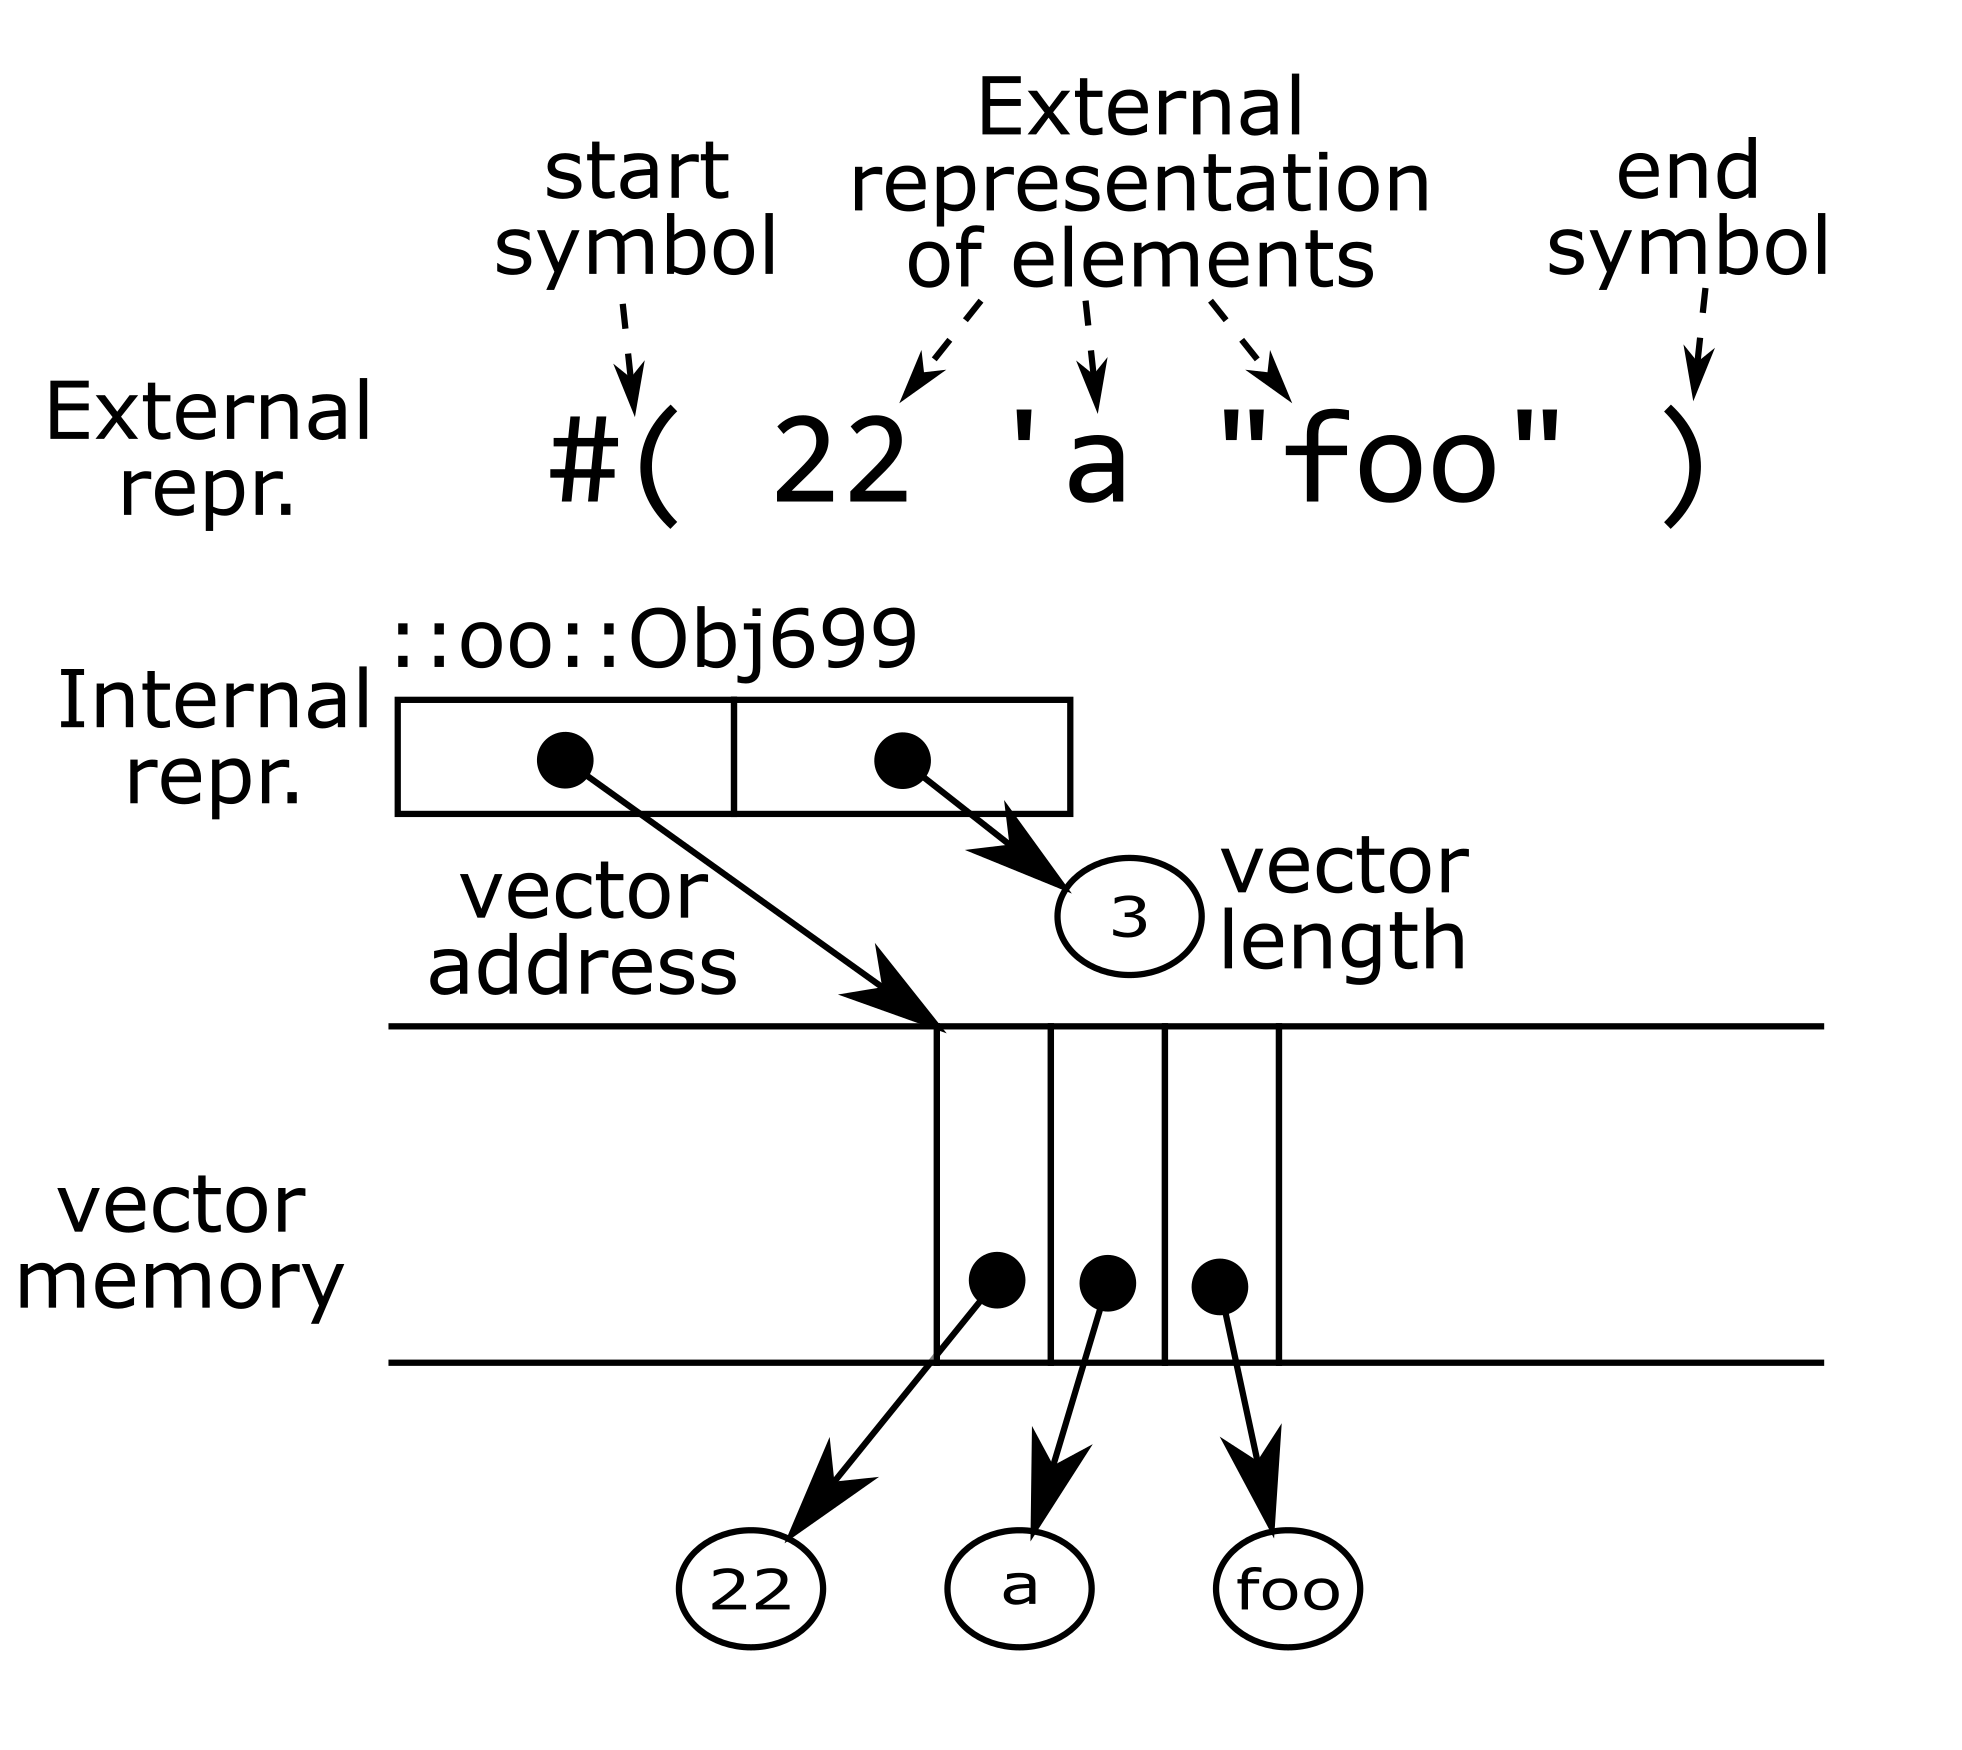
\includegraphics{images/vector-representation}

The \texttt{parse} procedure takes in the input buffer character by character, matching each character against a fitting external representation. When done, it creates a ConsTcl object, which is the internal representation of an expression. The object can then be passed to the evaluator.


Given a string, \texttt{parse} fills the input buffer. It then parses the input and produces the internal representation of an expression.


Example:

\begin{lstlisting}
% ::constcl::parse "(+ 2 3)"
::oo::Obj491
\end{lstlisting}

Here, \texttt{parse} parsed the external representation of a list with three elements, +, 2, and 3. It produced the expression that has an internal representation labeled \texttt{::oo::Obj491}. We will later meet procedures like \texttt{eval}, which transforms an expression into a value, and \texttt{write}, which prints a printed representation of expressions and values. Putting them together: we can see

\begin{lstlisting}
% ::constcl::write ::oo::Obj491
(+ 2 3)
% ::constcl::eval ::oo::Obj491
::oo::Obj494
% ::constcl::write ::oo::Obj494
5
\end{lstlisting}

Fortunately, we don't have to work at such a low level. We can use the \texttt{repl}\index{repl} instead:

\begin{lstlisting}
ConsTcl> (+ 2 3)
5
\end{lstlisting}

Then, parsing and evaluation and writing goes on in the background and the internal representations of expressions and values are hidden.


Anyway, here is how it really looks like. \texttt{::oo::Obj491} was just the head of the list.

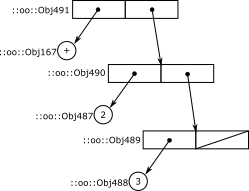
\includegraphics{images/intreplist.png}
\subsection{The parsing library}
\label{the-parsing-library}
\index{the parsing library}

\textbf{parse}


\texttt{parse} can be called with either a string input port or a Tcl or ConsTcl string (which \texttt{parse} uses to open a string input port). Once the input port is established, \texttt{parse} leaves control to \texttt{read-expr}.

\begin{tabular}{ |l l| }
\hline
\multicolumn{2}{|l|}{parse (internal)} \\
inp & a Tcl string or an input buffer \\
\textit{Returns:} & an expression \\
\hline
\end{tabular}
\index{parse}
\begin{lstlisting}
reg parse
 
proc ::constcl::parse {inp} {
  set c {}
  set unget {}
  if {[info object isa object $inp]} {
    if {[typeof? $inp IB] ne "#f"} {
      error "IB used"
    } elseif {[typeof? $inp StringInputPort] ne "#f"} {
      set port $inp
    } elseif {[typeof? $inp String] ne "#f"} {
      set port [::constcl::StringInputPort new [$inp value]]
    } else {
      ::error "Unknown object [$inp show]"
    }
  } else {
    # It's a Tcl string, we hope
    set port [StringInputPort new $inp]
  }
  set oldport $::constcl::Input_port
  set ::constcl::Input_port $port
  set expr [read-expr]
  set ::constcl::Input_port $oldport
  return $expr
}
\end{lstlisting}


\textbf{make-constant}


The \texttt{make-constant} helper procedure is called to set components of expressions to constants when read as a quoted literal.

\index{make-constant}
\begin{lstlisting}
proc ::constcl::make-constant {val} {
  if {[pair? $val] ne "#f"} {
    $val mkconstant
    make-constant [car $val]
    make-constant [cdr $val]
  } elseif {[null? $val] ne "#f"} {
    return #NIL
  } else {
    $val mkconstant
  }
}
\end{lstlisting}


\textbf{interspace}


The \texttt{interspace} helper procedure recognizes whitespace between value representations.

\index{interspace}
\begin{lstlisting}
proc ::constcl::interspace {c} {
  if {$c eq {} ||
    [::string is space $c] ||
    $c eq ";"} {
      return #t
    } else {
      return #f
    }
}
\end{lstlisting}


\textbf{character-check}


The \texttt{character-check} helper procedure compares a potential character constant to the valid kinds.

\begin{tabular}{ |l l| }
\hline
\multicolumn{2}{|l|}{character-check (internal)} \\
name & a Tcl string \\
\textit{Returns:} & a Tcl truth value (1 or 0) \\
\hline
\end{tabular}
\index{character-check}
\begin{lstlisting}
proc ::constcl::character-check {name} {
  if {[regexp {(?i)^#\\([[:graph:]]|space|newline)$} \
      $name]} {
    return #t
  } else {
    return #f
  }
}
\end{lstlisting}

\section{read}
\label{read}
\index{read}

\textbf{read}


The standard builtin \texttt{read} reads an input port approximately the same way that \texttt{parse} takes in an input buffer. The \texttt{read-} procedures parse their input and produce ConsTcl objects.


One can pass a port to \texttt{read}, in which case \texttt{read} sets the standard input port temporarily to the provided port. If not, \texttt{read} uses the standard input port (usually the keyboard).

\begin{tabular}{ |l l| }
\hline
\multicolumn{2}{|l|}{read (public)} \\
?port? & a port \\
\textit{Returns:} & an expression \\
\hline
\end{tabular}
\index{read}
\begin{lstlisting}
reg read
 
proc ::constcl::read {args} {
  set c {}
  set unget {}
  if {[llength $args]} {
    lassign $args port
  } else {
    set port $::constcl::Input_port
  }
  set oldport $::constcl::Input_port
  set ::constcl::Input_port $port
  set expr [read-expr]
  set ::constcl::Input_port $oldport
  return $expr
}
\end{lstlisting}


\textbf{read-expr}


The procedure \texttt{read-expr} reads input by reading the first available character and delegating to one of the more detailed reading procedures based on that, producing an expression of any kind. A Tcl character value can be passed to it, that character will be used first before reading from the input stream. If the end of file is encountered before an expression can be read in full, the procedure returns end of file\index{end of file}.

\begin{tabular}{ |l l| }
\hline
\multicolumn{2}{|l|}{read-expr (internal)} \\
?char? & a Tcl character \\
\textit{Returns:} & an expression or end of file \\
\hline
\end{tabular}
\index{read-expr}
\begin{lstlisting}
proc ::constcl::read-expr {args} {
  upvar c c unget unget
  if {[llength $args]} {
    lassign $args c
  } else {
    set c [readc]
  }
  set unget {}
  read-eof $c
  if {[::string is space $c] || $c eq ";"} {
    skip-ws
    read-eof $c
  }
  switch -regexp $c {
    {\"}          { read-string-expr }
    {\#}          { read-sharp }
    {\'}          { read-quoted-expr }
    {\(}          { read-pair-expr ")" }
    {\+} - {\-}   { read-plus-minus $c }
    {\,}          { read-unquoted-expr }
    {\.} {
        set x [Dot new]; set c [readc]; set x
    }
    {\:}          { read-object-expr }
    {\[}          { read-pair-expr "\]" }
    {\`}          { read-quasiquoted-expr }
    {\d}          { read-number-expr $c }
    {^$}          { return}
    {[[:graph:]]} { read-identifier-expr $c }
    default {
      read-eof $c
      ::error "unexpected character ($c)"
    }
  }
}
\end{lstlisting}


\texttt{readc} reads one character from the unget store if it isn't empty or else from the input stream. If the input stream is at end-of-file, an eof object is returned.

\begin{tabular}{ |l l| }
\hline
\multicolumn{2}{|l|}{readc (internal)} \\
\textit{Returns:} & a Tcl character or end of file \\
\hline
\end{tabular}
\index{readc}
\begin{lstlisting}
proc ::constcl::readc {} {
  upvar unget unget
  if {$unget ne {}} {
    set c $unget
    set unget {}
  } else {
    set c [$::constcl::Input_port get]
    if {[$::constcl::Input_port eof]} {
      return #EOF
    }
  }
  return $c
}
\end{lstlisting}


\texttt{read-find} reads ahead through whitespace to find a given character. Returns 1 if it has found the character, and 0 if it has stopped at some other character. Returns end of file if eof is encountered.

\begin{tabular}{ |l l| }
\hline
\multicolumn{2}{|l|}{read-find (internal)} \\
char & a Tcl character \\
\textit{Returns:} & a Tcl truth value (1 or 0) or end of file \\
\hline
\end{tabular}
\index{read-find}
\begin{lstlisting}
proc ::constcl::read-find {char} {
  upvar c c unget unget
  while {[::string is space -strict $c]} {
    set c [readc]
    read-eof $c
    set unget $c
  }
  return [expr {$c eq $char}]
}
\end{lstlisting}


\texttt{read-end} reads one character and returns 1 if it is an interspace character or an ending parenthesis or bracket. Otherwise it returns 0 or end-of-file if applicable. It ungets the character before returning.

\begin{tabular}{ |l l| }
\hline
\multicolumn{2}{|l|}{read-end (internal)} \\
->tbooleof &  \\
\hline
\end{tabular}
\index{read-end}
\begin{lstlisting}
proc ::constcl::read-end {} {
  upvar c c unget unget
  set c [readc]
  if {[interspace $c] ne "#f" || $c in {) ]} || $c eq "#EOF"} {
    set unget $c
    return 1
  } else {
    read-eof $c
    set unget $c
    return 0
  }
}
\end{lstlisting}


\texttt{skip-ws} skips whitespace and comments (the ; to end of line kind). Uses the shared \emph{c} character. It leaves the first character not to be skipped in \emph{c}.

\begin{tabular}{ |l l| }
\hline
\multicolumn{2}{|l|}{skip-ws (internal)} \\
\textit{Returns:} & nothing \\
\hline
\end{tabular}
\index{skip-ws}
\begin{lstlisting}
proc ::constcl::skip-ws {} {
  upvar c c unget unget
  while true {
    switch -regexp $c {
      {[[:space:]]} {
        set c [readc]
      }
      {;} {
        while {$c ne "\n" && $c ne "#EOF"}  {
          set c [readc]
        }
      }
      default {
        set unget $c
        return
      }
    }
  }
}
\end{lstlisting}


\texttt{read-eof} checks a number of objects for possible end-of-file objects. If it finds one, it returns \emph{from its caller} with the EOF value.

\begin{tabular}{ |l l| }
\hline
\multicolumn{2}{|l|}{read-eof (internal)} \\
args & some characters \\
\hline
\end{tabular}
\index{read-eof}
\begin{lstlisting}
proc ::constcl::read-eof {args} {
  foreach val $args {
    if {$val eq "#EOF"} {
      return -level 1 -code return #EOF
    }
  }
}
\end{lstlisting}


\textbf{read-string-expr}


\texttt{read-string-expr} is activated by \texttt{read-expr} when it reads a double quote. It collects characters until it reaches another (unescaped) double quote. It then returns a string expression--an immutable String\footnote{See page \pageref{strings}} object.

\begin{tabular}{ |l l| }
\hline
\multicolumn{2}{|l|}{read-string-expr (internal)} \\
\textit{Returns:} & a string or end of file \\
\hline
\end{tabular}
\index{read-string-expr}
\begin{lstlisting}
proc ::constcl::read-string-expr {} {
  upvar c c unget unget
  set str {}
  set c [readc]
  read-eof $c
  while {$c ne "\"" && $c ne "#EOF"} {
    if {$c eq "\\"} {
      ::append str $c
      set c [readc]
    }
    ::append str $c
    set c [readc]
  }
  if {$c eq "#EOF"} {
    error "bad string (no ending double quote)"
  }
  set c [readc]
  set expr [MkString $str]
  read-eof $expr
  $expr mkconstant
  return $expr
}
\end{lstlisting}


\textbf{read-sharp}


\texttt{read-sharp} is activated by \texttt{read-expr} when it reads a sharp sign (\texttt{\#}). It in turn either delegates to the vector reader or the character reader, or returns boolean literals.

\begin{tabular}{ |l l| }
\hline
\multicolumn{2}{|l|}{read-sharp (internal)} \\
\textit{Returns:} & a vector, boolean, or character value or end of file \\
\hline
\end{tabular}
\index{read-sharp}
\begin{lstlisting}
proc ::constcl::read-sharp {} {
  upvar c c unget unget
  set unget {}
  set c [readc]
  read-eof $c
  switch $c {
    (    { set n [read-vector-expr] }
    t    { if {[read-end]} {set n #t} }
    f    { if {[read-end]} {set n #f} }
    "\\" { set n [read-character-expr] }
    default {
      ::error "Illegal #-literal: #$c"
    }
  }
  return $n
}
\end{lstlisting}


\textbf{read-vector-expr}


\texttt{read-vector-expr} is activated by \texttt{read-sharp} and reads a number of expressions until it finds an ending parenthesis. It produces a vector expression and returns a Vector\footnote{See page \pageref{vectors}} object.

\begin{tabular}{ |l l| }
\hline
\multicolumn{2}{|l|}{read-vector-expr (internal)} \\
\textit{Returns:} & a vector or end of file \\
\hline
\end{tabular}
\index{read-vector-expr}
\begin{lstlisting}
proc ::constcl::read-vector-expr {} {
  upvar c c unget unget
  set res {}
  set c [readc]
  while {$c ne "#EOF" && $c ne ")"} {
    lappend res [read-expr $c]
    skip-ws
    read-eof $c
  }
  if {$c ne ")"} {
    ::error "Missing right paren. ($c)."
  }
  set expr [MkVector $res]
  read-eof $expr
  $expr mkconstant
  return $expr
}
\end{lstlisting}


\textbf{read-character-expr}


\texttt{read-character-expr} reads input, producing a character and returning a Char\footnote{See page \pageref{characters}} object.

\begin{tabular}{ |l l| }
\hline
\multicolumn{2}{|l|}{read-character-expr (internal)} \\
\textit{Returns:} & a character or end of file \\
\hline
\end{tabular}
\index{read-character-expr}
\begin{lstlisting}
proc ::constcl::read-character-expr {} {
  upvar c c unget unget
  set name "#\\"
  set c [readc]
  read-eof $c
  while {$c ni {) ]} && [::string is graph $c] && $c ne "#EOF"} {
    ::append name $c
    set c [readc]
  }
  check {character-check $name} {
      Invalid character constant $name
  }
  set expr [MkChar $name]
  read-eof $expr
  return $expr
}
\end{lstlisting}


\textbf{read-quoted-expr}


\texttt{read-quoted-expr} is activated by \texttt{read-expr} when reading a single quote ('). It then reads an entire expression beyond that, returning it wrapped in a list with \texttt{quote}. The quoted expression is made constant.

\begin{tabular}{ |l l| }
\hline
\multicolumn{2}{|l|}{read-quoted-expr (internal)} \\
\textit{Returns:} & an expression wrapped in the quote symbol or end of file \\
\hline
\end{tabular}
\index{read-quoted-expr}
\begin{lstlisting}
proc ::constcl::read-quoted-expr {} {
  upvar c c unget unget
  set unget {}
  set expr [read-expr]
  read-eof $expr
  make-constant $expr
  return [list [S quote] $expr]
}
\end{lstlisting}


\textbf{read-pair-expr}


The \texttt{read-pair-expr} procedure reads everything between two matching parentheses, or, as the case might be, brackets. It produces either an empty list, or a possibly recursive structure of Pair\footnote{See page \pageref{pairs-and-lists}} objects, either a proper list (one that ends in \#NIL), or an improper one (one that has an atom as its last member).

\begin{tabular}{ |l l| }
\hline
\multicolumn{2}{|l|}{read-pair-expr (internal)} \\
char & the terminating paren or bracket \\
\textit{Returns:} & a structure of pair expressions or end of file \\
\hline
\end{tabular}
\index{read-pair-expr}
\begin{lstlisting}
proc ::constcl::read-pair-expr {char} {
  upvar c c unget unget
  set unget {}
  set expr [read-pair $char]
  read-eof $expr
  if {$c ne $char} {
    if {$char eq ")"} {
      ::error \
        "Missing right paren. ($c)."
    } else {
      ::error \
        "Missing right bracket ($c)."
    }
  } else {
    set unget {}
    set c [readc]
  }
  return $expr
}
\end{lstlisting}


\texttt{read-pair} is a helper procedure that does the heavy lifting in reading a pair structure. First it checks if the list is empty, returning \#NIL in that case. Otherwise it reads the first element in the list and then repeatedly the rest of them. If it reads a Dot object, the following element to be read is the tail end of an improper list. When \texttt{read-pair} has reached the ending parenthesis or bracket, it conses up the elements starting from the last, and returns the head of the list.

\index{read-pair}
\begin{lstlisting}
proc ::constcl::read-pair {char} {
  upvar c c unget unget
  set c [readc]
  read-eof $c
  if {[read-find $char]} {
    # read right paren/brack
    #set c [readc]
    return #NIL
  }
  set a [read-expr $c]
  set res $a
  skip-ws
  set prev #NIL
  while {![read-find $char]} {
    set x [read-expr $c]
    skip-ws
    read-eof $c
    if {[dot? $x] ne "#f"} {
      set prev [read-expr $c]
      skip-ws
      read-eof $c
    } else {
      lappend res $x
    }
    if {[llength $res] > 99} break
  }
  # read right paren/brack
  foreach r [lreverse $res] {
    set prev [cons $r $prev]
  }
  return $prev
}
\end{lstlisting}


\textbf{read-plus-minus}


\texttt{read-plus-minus} is called when a plus or minus is found in the input stream. If the next character is a digit, it delegates to the number reader. Otherwise, it returns a \texttt{+} or \texttt{-} symbol.

\begin{tabular}{ |l l| }
\hline
\multicolumn{2}{|l|}{read-plus-minus (internal)} \\
\textit{Returns:} & either the symbols + or - or a number or end of file \\
\hline
\end{tabular}
\index{read-plus-minus}
\begin{lstlisting}
proc ::constcl::read-plus-minus {char} {
  upvar c c unget unget
  set unget {}
  set c [readc]
  read-eof $c
  if {[::string is digit -strict $c]} {
    set n [read-number-expr $c]
    read-eof $n
    if {$char eq "-"} {
      set n [- $n]
    }
    return $n
  } else {
    if {$char eq "+"} {
      return [S "+"]
    } else {
      return [S "-"]
    }
  }
}
\end{lstlisting}


\textbf{read-number-expr}


\texttt{read-number-expr} reads numerical input, both integers and floating point numbers. It actually takes in anything that starts out like a number and stops at whitespace or an ending parenthesis or bracket, and then it accepts or rejects the input by comparing it to a Tcl double. It returns a Number\footnote{See page \pageref{numbers}} object.

\begin{tabular}{ |l l| }
\hline
\multicolumn{2}{|l|}{read-number-expr (internal)} \\
?char? & a Tcl character \\
\textit{Returns:} & a number or end of file \\
\hline
\end{tabular}
\index{read-number-expr}
\begin{lstlisting}
proc ::constcl::read-number-expr {args} {
  upvar c c unget unget
  set unget {}
  if {[llength $args]} {
    lassign $args c
  } else {
    set c [readc]
  }
  read-eof $c
  while {[interspace $c] ne "#t" && $c ne "#EOF" &&
      $c ni {) ]}} {
    ::append num $c
    set c [readc]
  }
  set unget $c
  check {::string is double -strict $num} {
      Invalid numeric constant $num
  }
  set expr [N $num]
  return $expr
}
\end{lstlisting}


\textbf{read-unquoted-expr}


When a comma is found in the input stream, \texttt{read-unquoted-expr} is activated. If it reads an at-sign (\texttt{@}) it selects the symbol \texttt{unquote-splicing}, otherwise it selects the symbol \texttt{unquote}. Then it reads an entire expression and returns it wrapped in the selected symbol. Both of these expressions are only suppposed to occur inside a quasiquoted expression.

\begin{tabular}{ |l l| }
\hline
\multicolumn{2}{|l|}{read-unquoted-expr (internal)} \\
\textit{Returns:} & an expr. wr. in the unquote/-splicing symbol or end of file \\
\hline
\end{tabular}
\index{read-unquoted-expr}
\begin{lstlisting}
proc ::constcl::read-unquoted-expr {} {
  upvar c c unget unget
  set unget {}
  set c [readc]
  read-eof $c
  if {$c eq "@"} {
    set symbol "unquote-splicing"
    set expr [read-expr]
  } else {
    set symbol "unquote"
    set expr [read-expr $c]
  }
  read-eof $expr
  return [list [S $symbol] $expr]
}
\end{lstlisting}


\textbf{read-quasiquoted-expr}


\texttt{read-quasiquoted-expr} is activated when there is a backquote (\texttt{`}) in the input stream. It reads an entire expression and returns it wrapped in \texttt{quasiquote}.

\begin{tabular}{ |l l| }
\hline
\multicolumn{2}{|l|}{read-quasiquoted-expr (internal)} \\
\textit{Returns:} & an expr. wr. in the quasiquote symbol or end of file \\
\hline
\end{tabular}
\index{read-quasiquoted-expr}
\begin{lstlisting}
proc ::constcl::read-quasiquoted-expr {} {
  upvar c c unget unget
  set unget {}
  set expr [read-expr]
  skip-ws
  read-eof $expr
  make-constant $expr
  return [list [S "quasiquote"] $expr]
}
\end{lstlisting}


\textbf{read-identifier-expr}


\texttt{read-identifier-expr} is activated for "anything else", and takes in characters until it finds whitespace or an ending parenthesis or bracket. It checks the input against the rules for identifiers, accepting or rejecting it with an error message. It returns a Symbol\footnote{See page \pageref{symbols}} object.

\begin{tabular}{ |l l| }
\hline
\multicolumn{2}{|l|}{read-identifier-expr (internal)} \\
?char? & a Tcl character \\
\textit{Returns:} & a symbol or end of file \\
\hline
\end{tabular}
\index{read-identifier-expr}
\begin{lstlisting}
proc ::constcl::read-identifier-expr {args} {
  upvar c c unget unget
  set unget {}
  if {[llength $args]} {
    lassign $args c
  } else {
    set c [readc]
  }
  read-eof $c
  set name {}
  while {[::string is graph -strict $c]} {
    if {$c eq "#EOF" || $c in {) \]}} {
      break
    }
    ::append name $c
    set c [readc]
  }
  if {$c ne "#EOF"} {
    set unget $c
  }
  read-eof $name
  # idcheck throws error if invalid identifier
  idcheck $name
  return [S $name]
}
\end{lstlisting}


\textbf{read-object-expr}


A non-standard extension, \texttt{read-object-expr} reads a ConsTcl object of any kind and passes its name along.

\begin{tabular}{ |l l| }
\hline
\multicolumn{2}{|l|}{read-object-expr (internal)} \\
\textit{Returns:} & a ConsTcl object or end of file \\
\hline
\end{tabular}
\index{read-object-expr}
\begin{lstlisting}
proc ::constcl::read-object-expr {} {
  upvar c c unget unget
  # first colon has already been read
  foreach ch [split ":oo::Obj" {}] {
    set c [readc]
    read-eof $c
    if {$c ne $ch} {
      error "bad object name"
    }
  }
  set res "::oo::Obj"
  set c [readc]
  read-eof $c
  while {[::string is digit $c]} {
    ::append res $c
    set c [readc]
    read-eof $c
  }
  set unget $c
  return $res
}
\end{lstlisting}

\chapter{Evaluation}
\label{evaluation}

The second thing an interpreter must be able to do is to reduce expressions to their \emph{normal form}, or \emph{evaluate}\index{eval}\index{evaluator} them. As an example, 2 + 6 and 8 are two expressions that have the same value, but the latter is in normal form (can't be reduced further) and the former is not.

\section{Syntactic forms}
\label{syntactic-forms}
\index{syntactic forms}

There are nine diffent forms or classes of expressions in Lisp. The evaluator recognizes each one by its internal representation and chooses the appropriate process to evaluate them. The nine forms will be described in the following sections.



\textbf{eval}


The heart of the Lisp interpreter, \texttt{eval} takes a Lisp expression and processes it according to its syntactic form.


\texttt{eval} also does two kinds of rewriting of expressions: 1) \emph{macro expansion} on a non-atomic expression into a more concrete expression. See the part about macros\footnote{See page \pageref{macros}} below, and 2) resolving \emph{local defines}, acting on expressions of the form \texttt{(begin (define ...} when in a local environment. See the part about resolving local defines\footnote{See page \pageref{resolving-local-defines}}.

\begin{tabular}{ |l l| }
\hline
\multicolumn{2}{|l|}{eval (public)} \\
expr & an expression \\
env & an environment \\
\textit{Returns:} & a Lisp value \\
\hline
\end{tabular}
\index{eval}
\begin{lstlisting}
reg eval
 
proc ::constcl::eval \
  {expr {env ::constcl::global_env}} {
  if {[symbol? $expr] ne "#f"} {
    lookup $expr $env
  } elseif {[null? $expr] ne "#f" ||
    [atom? $expr] ne "#f"} {
    set expr
  } else {
    while {[[car $expr] name] in
      $::constcl::macrolist} {
      set expr [expand-macro $expr $env]
    }
    set op [car $expr]
    set args [cdr $expr]
    if {$env ne "::constcl::global_env" &&
      [$op name] eq "begin" &&
      ([pair? [car $args]] ne "#f" &&
      [[caar $args] name] eq "define")} {
      set expr [resolve-local-defines $args]
      set op [car $expr]
      set args [cdr $expr]
    }
    switch [$op name] {
      quote {
        car $args
      }
      if {
        if {[eval [car $args] $env] ne "#f"} \
          {eval [cadr $args] $env} \
          {eval [caddr $args] $env}
      }
      begin {
        /begin $args $env
      }
      define {
        /define [car $args] [
          eval [cadr $args] $env] $env
      }
      set! {
        /set! [car $args] [
          eval [cadr $args] $env] $env 
      }
      lambda {
        /lambda [car $args] [
          cdr $args] $env
      }
      default {
        invoke [eval $op $env] [
          eval-list $args $env]
      }
    }
  }
}
\end{lstlisting}

\subsection{Variable reference}
\label{variable-reference}
\index{variable reference}

E{Example: \texttt{r} => 10 (a symbol \texttt{r} is evaluated to 10)}


A variable\index{variable} is an identifier (symbol) bound to a location in the environment. If an expression consists of the identifier it is evaluated to the value stored in that location. This is handled by the helper procedure \texttt{lookup}. It searches the environment chain for the identifier, and returns the value stored in the location it is bound to. It is an error to do lookup on an unbound symbol.


\textbf{lookup}

\begin{tabular}{ |l l| }
\hline
\multicolumn{2}{|l|}{lookup (internal)} \\
sym & a symbol \\
env & an environment \\
\textit{Returns:} & a Lisp value \\
\hline
\end{tabular}
\index{lookup}
\begin{lstlisting}
proc ::constcl::lookup {sym env} {
  [$env find $sym] get $sym
}
\end{lstlisting}

\subsection{Constant literal}
\label{constant-literal}
\index{constant literal}

E{Example: \texttt{99} => 99 (a number evaluates to itself)}


Not just numbers but booleans, characters, strings, and vectors evaluate to themselves, to their innate value. Because of this, they are called autoquoting types (see next paragraph).


\subsection{Quotation}
\label{quotation}
\index{quotation}

E{Example: \texttt{(quote r)} => \texttt{r} (quotation makes the symbol evaluate to itself, like a constant)}


According to the rules of variable reference, a symbol evaluates to its stored value. Well, sometimes one wishes to use the symbol itself as a value. That is what quotation is for. \texttt{(quote x)} evaluates to the symbol x itself and not to any value that might be stored under it. This is so common that there is a shorthand notation for it: \texttt{'x} is interpreted as \texttt{(quote x)} by the Lisp reader.


\subsection{Conditional}
\label{conditional}
\index{conditional}

E{Example: \texttt{(if (> 99 100) (* 2 2) (+ 2 4))} => 6}


The conditional form \texttt{if} evaluates a Lisp list of three expressions. The first, the \emph{condition}, is evaluated first. If it evaluates to anything other than \texttt{\#f} (false), the second expression (the \emph{consequent}) is evaluated and the value returned. Otherwise, the third expression (the \emph{alternate}) is evaluated and the value returned. One of the two latter expressions will be evaluated, and the other will remain unevaluated.


\textbf{/if}

\begin{tabular}{ |l l| }
\hline
\multicolumn{2}{|l|}{/if (internal)} \\
condition & an expression \\
consequent & an expression \\
alternate & an expression \\
\textit{Returns:} & a Lisp value \\
\hline
\end{tabular}
\index{/if}
\begin{lstlisting}
proc ::constcl::/if {cond conseq altern} {
  if {[uplevel $cond] ne "#f"} {
    uplevel $conseq
  } {
    uplevel $altern
  }
}
\end{lstlisting}

\subsection{Sequence}
\label{sequence}
\index{sequence}

E{Example: \texttt{(begin (define r 10) (* r r))} => 100}


When expressions are evaluated in sequence, the order is important for two reasons. If the expressions have any side effects, they happen in the same order of sequence. Also, if expressions are part of a pipeline of calculations, then they need to be processed in the order of that pipeline. The \texttt{/begin} helper procedure takes a Lisp list of expressions and evaluates them in sequence, returning the value of the last one.


\textbf{/begin}

\begin{tabular}{ |l l| }
\hline
\multicolumn{2}{|l|}{/begin (internal)} \\
exps & a Lisp list of expressions \\
env & an environment \\
\textit{Returns:} & a Lisp value \\
\hline
\end{tabular}
\index{/begin}
\begin{lstlisting}
proc ::constcl::/begin {exps env} {
  /if {pair? $exps} {
    /if {pair? [cdr $exps]} {
      eval [car $exps] $env
      return [/begin [cdr $exps] $env]
    } {
      return [eval [car $exps] $env]
    }
  } {
    return #NIL
  }
}
\end{lstlisting}

\subsection{Definition}
\label{definition}
\index{definition}

E{Example: \texttt{(define r 10)} => ... (a definition doesn't evaluate to anything)}


We've already seen the relationship between symbols and values. A symbol is bound to a value (or rather to the location the value is in), creating a variable, through definition. The \texttt{/define} helper procedure adds a variable to the current environment. It first checks that the symbol name is a valid identifier, then it updates the environment with the new binding.


\textbf{/define}

\begin{tabular}{ |l l| }
\hline
\multicolumn{2}{|l|}{/define (internal)} \\
sym & a symbol \\
val & a Lisp value \\
env & an environment \\
\textit{Returns:} & nothing \\
\hline
\end{tabular}
\index{/define}
\begin{lstlisting}
proc ::constcl::/define {sym val env} {
  varcheck [idcheck [$sym name]]
  $env set $sym $val
  return
}
\end{lstlisting}

\subsection{Assignment}
\label{assignment}
\index{assignment}

**Example: \texttt{(set! r 20)} => 20 (\texttt{r} is a bound symbol, so it's allowed to assign to it)**


Once a variable has been created, the value at the location it is bound to can be changed (hence the name "variable", something that can be modified). The process is called assignment. The \texttt{/set!} helper does assignment: it modifies an existing variable that is bound somewhere in the environment chain. It finds the variable's environment and updates the binding. It returns the value, so calls to \texttt{set!} can be chained: \texttt{(set! foo (set! bar 99))} sets both variables to 99. By Scheme convention, procedures that modify variables have "!" at the end of their name.


\textbf{/set!}

\begin{tabular}{ |l l| }
\hline
\multicolumn{2}{|l|}{/set! (internal)} \\
var & a bound symbol \\
val & a Lisp value \\
env & an environment \\
\textit{Returns:} & a Lisp value \\
\hline
\end{tabular}
\index{/set!}
\begin{lstlisting}
proc ::constcl::/set! {var val env} {
  [$env find $var] set $var $val
  set val
}
\end{lstlisting}

\subsection{Procedure definition}
\label{procedure-definition}
\index{procedure definition}

**Example: \texttt{(lambda (r) (* r r))} => ::oo::Obj3601 (it will be a different object each time)**


In Lisp, procedures are values just like numbers or characters. They can be defined as the value of a symbol, passed to other procedures, and returned from procedures. One diffence from most values is that procedures need to be defined. Two questions must answered: what is the procedure meant to do? The code that does that will form the body of the procedure. Also, what, if any, items of data will have to be provided to the procedure to make it possible to calculate its result?


As an example, imagine that we want to have a procedure that calculates the square (\texttt{x · x}) of a given number. In Lisp, expressions are written with the operator first and then the operands: \texttt{(* x x)}. That is the body of the procedure. Now, what data will we have to provide to the procedure to make it work? A value stored in the variable \texttt{x} will do. It's only a single variable, but by custom we need to put it in a list: \texttt{(x)}. The operator that defines procedures is called \texttt{lambda}\index{lambda}, and we define the function with \texttt{(lambda (x) (* x x))}.


One more step is needed before we can use the procedure. It must have a name. We could define it like this: \texttt{(define square (lambda (x) (* x x)))} but there is actually a shortcut notation for it: \texttt{(define (square x) (* x x))}.


Now, \texttt{square} is pretty tame. How about the \texttt{hypotenuse} procedure? \texttt{(define (hypotenuse a b) (sqrt (+ (square a) (square b))))}. It calculates the square root of the sum of two squares.


Under the hood, the helper \texttt{/lambda} makes a Procedure\footnote{See page \pageref{control}} object. First it needs to convert the Lisp list \texttt{body}. It is packed inside a \texttt{begin} if it has more than one expression, and taken out of its list if not. The Lisp list \texttt{formals} is passed on as it is.


A Scheme formals list\index{formals list} is either:


* An \emph{empty list}, \texttt{()}, meaning that no arguments are accepted, * A \emph{proper list}, \texttt{(a b c)}, meaning it accepts three arguments, one in each symbol, * A \emph{symbol}, \texttt{a}, meaning that all arguments go into \texttt{a}, or * A \emph{dotted list}, \texttt{(a b . c)}, meaning that two arguments go into \texttt{a} and \texttt{b}, and the rest into \texttt{c}.


\textbf{/lambda}

\begin{tabular}{ |l l| }
\hline
\multicolumn{2}{|l|}{/lambda (internal)} \\
formals & a Scheme formals list \\
body & a Lisp list of expressions \\
env & an environment \\
\textit{Returns:} & a procedure \\
\hline
\end{tabular}
\index{/lambda}
\begin{lstlisting}
proc ::constcl::/lambda {formals body env} {
  if {[[length $body] value] > 1} {
    set body [cons [S begin] $body]
  } else {
    set body [car $body]
  }
  return [MkProcedure $formals $body $env]
}
\end{lstlisting}

\subsection{Procedure call}
\label{procedure-call}
\index{procedure call}

E{Example: \texttt{(+ 1 6)} => 7}


Once we have procedures, we can call them to have their calculations performed and yield results. The procedure name is put in the operator position at the front of a list, and the operands follow in the rest of the list. Our \texttt{square} procedure would be called for instance like this: \texttt{(square 11)}, and it will return 121.


\texttt{invoke} arranges for a procedure to be called with each of the values in the \emph{argument list} (the list of operands). It checks if pr really is a procedure, and determines whether to call pr as an object or as a Tcl command.


\textbf{invoke}

\begin{tabular}{ |l l| }
\hline
\multicolumn{2}{|l|}{invoke (internal)} \\
pr & a procedure \\
vals & a Lisp list of Lisp values \\
\textit{Returns:} & what pr returns \\
\hline
\end{tabular}
\index{invoke}
\begin{lstlisting}
proc ::constcl::invoke {pr vals} {
  check {procedure? $pr} {
    PROCEDURE expected\n([$pr show] val ...)
  }
  if {[info object isa object $pr]} {
    $pr call {*}[splitlist $vals]
  } else {
    $pr {*}[splitlist $vals]
  }
}
\end{lstlisting}


\textbf{splitlist}


\texttt{splitlist} converts a Lisp list to a Tcl list with Lisp objects.

\begin{tabular}{ |l l| }
\hline
\multicolumn{2}{|l|}{splitlist (internal)} \\
vals & a Lisp list of Lisp values \\
\textit{Returns:} & a Tcl list of Lisp values \\
\hline
\end{tabular}
\index{splitlist}
\begin{lstlisting}
proc ::constcl::splitlist {vals} {
  set result {}
  while {[pair? $vals] ne "#f"} {
    lappend result [car $vals]
    set vals [cdr $vals]
  }
  return $result
}
\end{lstlisting}


\textbf{eval-list}


\texttt{eval-list} successively evaluates the elements of a Lisp list and returns the collected results as a Lisp list.

\begin{tabular}{ |l l| }
\hline
\multicolumn{2}{|l|}{eval-list (internal)} \\
exps & a Lisp list of expressions \\
env & an environment \\
\textit{Returns:} & a Lisp list of Lisp values \\
\hline
\end{tabular}
\index{eval-list}
\begin{lstlisting}
proc ::constcl::eval-list {exps env} {
  # don't convert to /if, it breaks (fact 100)
  if {[pair? $exps] ne "#f"} {
    return [cons [eval [car $exps] $env] \
      [eval-list [cdr $exps] $env]]
  } {
    return #NIL
  }
}
\end{lstlisting}
\section{Macros}
\label{macros}
\index{macros}


\textbf{expand-macro}


Macros that rewrite expressions into other, more concrete expressions is one of Lisp's strong points. This interpreter does macro expansion, but the user can't define new macros--the ones available are hardcoded in the code below.


\texttt{expand-macro} takes an expression and an environment as a parameter. First, the operator (\texttt{op}) and operands (\texttt{args}) are extracted to check if expansion is necessary (the operator \texttt{car}, for historical reasons, stands for the first element of a list, while \texttt{cdr} stands for the rest of the elements after the first in a list). If the operator is the symbol \texttt{define} and the first of the operands is something other than a Pair, then expansion is unnecessary and the procedure returns with a code to break the while loop in \texttt{eval}.


The operator's symbol name is then used to select the right expansion procedure, and the whole expression and the environment is passed to it. In the end, the expanded expression is passed back to \texttt{eval}.

\begin{tabular}{ |l l| }
\hline
\multicolumn{2}{|l|}{expand-macro (internal)} \\
expr & an expression \\
env & an environment \\
\textit{Returns:} & an expression \\
\hline
\end{tabular}
\index{expand-macro}
\begin{lstlisting}
proc ::constcl::expand-macro {expr env} {
  set op [car $expr]
  set args [cdr $expr]
  if {[$op name] eq "define" &&
      [pair? [car $args]] eq "#f"} {
    return -code break
  }
  return [expand-[$op name] $expr $env]
}
\end{lstlisting}


\textbf{expand-and}


\texttt{expand-and} expands the \texttt{and} macro. It returns a \texttt{begin}-expression if the macro has 0 or 1 elements, and a nested \texttt{if} construct otherwise. \texttt{S begin} stands for "the symbol begin".

\begin{tabular}{ |l l| }
\hline
\multicolumn{2}{|l|}{expand-and (internal)} \\
expr & an expression \\
env & an environment \\
\textit{Returns:} & an expression \\
\hline
\end{tabular}
\index{expand-and}
\begin{lstlisting}
regmacro and
 
proc ::constcl::expand-and {expr env} {
  set tail [cdr $expr]
  if {[[length $tail] numval] == 0} {
    list [S begin] #t
  } elseif {[[length $tail] numval] == 1} {
    cons [S begin] $tail
  } else {
    do-and $tail #t $env
  }
}
\end{lstlisting}

\subsubsection{Quasiquote: an aside}
\label{quasiquote:-an-aside}

In this and many other macro expanders I use a quasiquote construct to lay out how the is to be expanded. A quasiquote starts with a backquote (\texttt{`}) instead of the single quote that precedes regular quoted material. A quasiquote allows for "unquoting" of selected parts: this is notated with a comma (\texttt{,}). \texttt{`(foo ,bar baz)} is very nearly the same as \texttt{('foo bar 'baz)}, except that the list structure itself is constant in a quasiquote. Anyway, in both cases \texttt{foo} and \texttt{baz} are constants while \texttt{bar} is a variable which will be evaluated. Like in \texttt{do-and} here, a quasiquote serves well as a templating mechanism. The variables in the quasiquote need to be a part of the environment in which the quasiquote is expanded: I use \texttt{/define} to bind them in a temporary environment.

\begin{tabular}{ |l l| }
\hline
\multicolumn{2}{|l|}{do-and (internal)} \\
tail & an expression tail \\
prev & an expression \\
env & an environment \\
\textit{Returns:} & an expression \\
\hline
\end{tabular}
\index{do-and}
\begin{lstlisting}
proc ::constcl::do-and {tail prev env} {
  set env [Environment new #NIL {} $env]
  if {[[length $tail] numval] == 0} {
    return $prev
  } else {
    /define [S first] [car $tail] $env
    /define [S rest] [do-and [cdr $tail] \
        [car $tail] $env] $env
    set qq "`(if ,first ,rest #f)"
    return [expand-quasiquote [parse $qq] $env]
  }
}
\end{lstlisting}


\textbf{expand-case}


The body of the \texttt{case} form consists of a key-expression and a number of clauses. Each clause has a list of values and a body. If the key-expression evaluates to a value that occurs in one of the value-lists (considered in order), that clause's body is evaluated and all other clauses are ignored.


The \texttt{case} macro is expanded by \texttt{expand-case}. It expands to \texttt{'()} if there are no clauses (left), and to nested \texttt{if} constructs if there are some.

\subsubsection{caar, cadr, cdar, and the rest, an aside}
\label{caar,-cadr,-cdar,-and-the-rest,-an-aside}


The \texttt{do-case} procedure uses extensions of the \texttt{car}/\texttt{cdr} operators like \texttt{caar} and \texttt{cdar}. \texttt{car}/\texttt{cdr} notation gets really powerful when combined to form operators from \texttt{caar} to \texttt{cddddr}. One can read \texttt{caar L} as "the first element of the first element of L", implying that the first element of \texttt{L} is a list. \texttt{cdar L} is "the rest of the elements of the first element of L", and \texttt{cadr L} is "the first element of the rest of the elements of L" or in layman's terms, the second element of L.

\begin{tabular}{ |l l| }
\hline
\multicolumn{2}{|l|}{expand-case (internal)} \\
expr & an expression \\
env & an environment \\
\textit{Returns:} & an expression \\
\hline
\end{tabular}
\index{expand-case}
\begin{lstlisting}
regmacro case
 
proc ::constcl::expand-case {expr env} {
  set tail [cdr $expr]
  do-case [car $tail] [cdr $tail] $env
}
 
proc ::constcl::do-case {keyexpr clauses env} {
  if {[eq? [length $clauses] #0] ne "#f"} {
    return [parse "'()"]
  } else {
    set keyl [caar $clauses]
    set body [cdar $clauses]
    set keyl [list [S memv] $keyexpr \
        [list [S quote] $keyl]]
    # if this is the last clause...
    if {[eq? [length $clauses] #1] ne "#f"} {
      # ...allow 'else' in the condition
      if {[eq? [caar $clauses] [S else]] ne "#f"} {
        set keyl #t
      }
    }
    set env [Environment new #NIL {} $env]
    /define [S keyl] $keyl $env
    /define [S body] $body $env
    /define [S rest] [
      do-case $keyexpr [cdr $clauses] $env] $env
    set qq "`(if ,keyl
               (begin ,@body)
               ,rest)"
    return [expand-quasiquote [parse $qq] $env]
  }
}
\end{lstlisting}


\textbf{expand-cond}


The \texttt{cond} form has a list of clauses, each with a predicate and a body. The clauses is considered in order, and if a predicate evaluates to something other than \texttt{\#f} the body is evaluated and the remaining clauses are ignored.


The \texttt{cond} macro is expanded by \texttt{expand-cond}. It expands to \texttt{'()} if there are no clauses (left), and to nested \texttt{if} constructs if there are some.

\begin{tabular}{ |l l| }
\hline
\multicolumn{2}{|l|}{expand-cond (internal)} \\
expr & an expression \\
env & an environment \\
\textit{Returns:} & an expression \\
\hline
\end{tabular}
\index{expand-cond}
\begin{lstlisting}
regmacro cond
 
proc ::constcl::expand-cond {expr env} {
  return [do-cond [cdr $expr] $env]
}
 
proc ::constcl::do-cond {tail env} {
  set clauses $tail
  if {[eq? [length $clauses] #0] ne "#f"} {
    return [parse "'()"]
  } else {
    set pred [caar $clauses]
    set body [cdar $clauses]
    if {[symbol? [car $body]] ne "#f" &&
        [[car $body] name] eq "=>"} {
      set body [cddar $clauses]
    }
    # if this is the last clause...
    if {[eq? [length $clauses] #1] ne "#f"} {
      # ...allow 'else' in the predicate
      if {[eq? $pred [S else]] ne "#f"} {
        set pred #t
      }
    }
    if {[null? $body] ne "#f"} {
        set body $pred
    }
    set env [Environment new #NIL {} $env]
    /define [S pred] $pred $env
    /define [S body] $body $env
    /define [S rest] [
      do-cond [cdr $clauses] $env] $env
    set qq "`(if ,pred
               (begin ,@body)
               ,rest)"
    return [expand-quasiquote [parse $qq] $env]
  }
}
\end{lstlisting}


\textbf{expand-define}


\texttt{define} has two variants, one of which requires some rewriting. It's the one with an implied \texttt{lambda} call, the one that defines a procedure.


(define (\emph{symbol} \emph{formals}) \emph{body})


is transformed into


(define \emph{symbol} (lambda \emph{formals} \emph{body}))


which conforms better to \texttt{eval}'s standard of (define \emph{symbol} \emph{value}).

\begin{tabular}{ |l l| }
\hline
\multicolumn{2}{|l|}{expand-define (internal)} \\
expr & an expression \\
env & an environment \\
\textit{Returns:} & an expression \\
\hline
\end{tabular}
\index{expand-define}
\begin{lstlisting}
regmacro define
 
proc ::constcl::expand-define {expr env} {
  set tail [cdr $expr]
  set env [::constcl::Environment new #NIL {} $env]
  /define [S tail] $tail $env
  set qq "`(define ,(caar tail)
             (lambda ,(cdar tail) ,@(cdr tail)))"
  return [expand-quasiquote [parse $qq] $env]
}
\end{lstlisting}


\textbf{expand-del!}


The macro \texttt{del!} updates a property list. It removes a key-value pair if the key is present, or leaves the list untouched if it isn't.

\begin{tabular}{ |l l| }
\hline
\multicolumn{2}{|l|}{expand-del! (internal)} \\
expr & an expression \\
env & an environment \\
\textit{Returns:} & an expression \\
\hline
\end{tabular}
\index{expand-del!}
\begin{lstlisting}
regmacro del!
 
proc ::constcl::expand-del! {expr env} {
  set tail [cdr $expr]
  set env [Environment new #NIL {} $env]
  if {[null? $tail] ne "#f"} {
    ::error "too few arguments, 0 of 2"
  }
  /define [S listname] [car $tail] $env
  if {[null? [cdr $tail]] ne "#f"} {
    ::error "too few arguments, 1 of 2"
  }
  /define [S key] [cadr $tail] $env
  set qq "`(set! ,listname
             (delete! ,listname ,key))"
  return [expand-quasiquote [parse $qq] $env]
}
\end{lstlisting}


\textbf{expand-for}


The \texttt{expand-for} procedure expands the \texttt{for} macro. It returns a \texttt{begin} construct containing the iterations of each clause (multiple clauses weren't implemented, but I brought up my strongest brain cells and they did it).

\begin{tabular}{ |l l| }
\hline
\multicolumn{2}{|l|}{for-seq (internal)} \\
seq & a Lisp value \\
env & an environment \\
\textit{Returns:} & a Tcl list of Lisp values \\
\hline
\end{tabular}
\index{for-seq}
\begin{lstlisting}
regmacro for
 
proc ::constcl::for-seq {seq env} {
  if {[number? $seq] ne "#f"} {
    set seq [in-range $seq]
  } else {
    set seq [eval $seq $env]
  }
  # make it a Tcl list, one way or another
  if {[list? $seq] ne "#f"} {
    set seq [splitlist $seq]
  } elseif {[string? $seq] ne "#f"} { 
    set seq [lmap c [split [$seq value] {}] {
      MkChar #\\$c
    }]
  } elseif {[vector? $seq] ne "#f"} {
    set seq [$seq value]
  }
}
\end{lstlisting}
\begin{tabular}{ |l l| }
\hline
\multicolumn{2}{|l|}{do-for (internal)} \\
tail & an expression tail \\
env & an environment \\
\textit{Returns:} & a Tcl list of expressions \\
\hline
\end{tabular}
\index{do-for}
\begin{lstlisting}
proc ::constcl::do-for {tail env} {
  # make clauses a Tcl list
  set clauses [splitlist [car $tail]]
  set body [cdr $tail]
  set data [dict create]
  set length 0
  foreach clause $clauses {
    set id [car $clause]
    set iter [for-seq [cadr $clause] $env]
    set length [llength $iter]
    # save every id and step of the iteration
    for {set i 0} {$i < $length} {incr i} {
        dict set data $id $i [lindex $iter $i]
    }
  }
  set res {}
  # for every step of the iteration...
  for {set i 0} {$i < $length} {incr i} {
    set decl {}
    # retrieve the ids
    foreach id [dict keys $data] {
      # list the id and the step
      lappend decl [
        list $id [dict get $data $id $i]]
    }
    # add to the structure of let constructs
    lappend res [list [S let] [
        list {*}$decl] {*}[splitlist $body]]
  }
  return $res
}
\end{lstlisting}
\begin{tabular}{ |l l| }
\hline
\multicolumn{2}{|l|}{expand-for (internal)} \\
expr & an expression \\
env & an environment \\
\textit{Returns:} & an expression \\
\hline
\end{tabular}
\index{expand-for}
\begin{lstlisting}
proc ::constcl::expand-for {expr env} {
  set tail [cdr $expr]
  set res [do-for $tail $env]
  lappend res [parse "'()"]
  return [list [S begin] {*}$res]
}
\end{lstlisting}


\textbf{expand-for/and}


The \texttt{expand-for/and} procedure expands the \texttt{for/and} macro. It returns an \texttt{and} construct containing the iterations of the clauses.

\begin{tabular}{ |l l| }
\hline
\multicolumn{2}{|l|}{expand-for/and (internal)} \\
expr & an expression \\
env & an environment \\
\textit{Returns:} & an expression \\
\hline
\end{tabular}
\index{expand}
\begin{lstlisting}
regmacro for/and
 
proc ::constcl::expand-for/and {expr env} {
  set tail [cdr $expr]
  set res [do-for $tail $env]
  return [list [S and] {*}$res]
}
\end{lstlisting}


\textbf{expand-for/list}


The \texttt{expand-for/list} procedure expands the \texttt{for/list} macro. It returns a \texttt{list} construct containing the iterations of each clause.

\begin{tabular}{ |l l| }
\hline
\multicolumn{2}{|l|}{expand for/list (internal)} \\
expr & an expression \\
env & an environment \\
\textit{Returns:} & an expression \\
\hline
\end{tabular}
\index{expand-for/list}
\begin{lstlisting}
regmacro for/list
 
proc ::constcl::expand-for/list {expr env} {
  set tail [cdr $expr]
  set res [do-for $tail $env]
  return [list [S list] {*}$res]
}
\end{lstlisting}


\textbf{expand-for/or}


The \texttt{expand-for/or} procedure expands the \texttt{for/or} macro. It returns an \texttt{or} construct containing the iterations of each clause.

\begin{tabular}{ |l l| }
\hline
\multicolumn{2}{|l|}{expand-for/or (internal)} \\
expr & an expression \\
env & an environment \\
\textit{Returns:} & an expression \\
\hline
\end{tabular}
\index{expand-for/or}
\begin{lstlisting}
regmacro for/or
 
proc ::constcl::expand-for/or {expr env} {
  set tail [cdr $expr]
  set res [do-for $tail $env]
  return [list [S or] {*}$res]
}
\end{lstlisting}


\textbf{expand-let}


\texttt{expand-let} expands the named \texttt{let} and 'regular' \texttt{let} macros. They ultimately expand to \texttt{lambda} constructs.

\begin{tabular}{ |l l| }
\hline
\multicolumn{2}{|l|}{expand-let (internal)} \\
expr & an expression \\
env & an environment \\
\textit{Returns:} & an expression \\
\hline
\end{tabular}
\index{expand-let}
\begin{lstlisting}
regmacro let
 
proc ::constcl::expand-let {expr env} {
  set tail [cdr $expr]
  set env [Environment new #NIL {} $env]
  if {[symbol? [car $tail]] ne "#f"} {
    # named let
    set variable [car $tail]
    set bindings [cadr $tail]
    set body [cddr $tail]
    set vars [dict create $variable #f]
    parse-bindings vars $bindings
    /define [S decl] [list {*}[dict values [
      dict map {k v} $vars {list $k $v}]]] $env
    /define [S variable] $variable $env
    /define [S varlist] [list {*}[lrange [
      dict keys $vars] 1 end]] $env
    /define [S body] $body $env
    /define [S call] [list {*}[
      dict keys $vars]] $env
    set qq "`(let ,decl
               (set!
                 ,variable
                 (lambda ,varlist ,@body)) ,call)"
    return [expand-quasiquote [parse $qq] $env]
  } else {
    # regular let
    set bindings [car $tail]
    set body [cdr $tail]
    set vars [dict create]
    parse-bindings vars $bindings
    /define [S varlist] [list {*}[
      dict keys $vars]] $env
    /define [S body] $body $env
    /define [S vallist] [list {*}[
      dict values $vars]] $env
    set qq "`((lambda ,varlist ,@body)
               ,@vallist)"
    return [expand-quasiquote [parse $qq] $env]
  }
}
 
proc ::constcl::parse-bindings {name bindings} {
  upvar $name vars
  foreach binding [splitlist $bindings] {
    set var [car $binding]
    set val [cadr $binding]
    if {$var in [dict keys $vars]} {
        ::error "'$var' occurs more than once"
    }
    dict set vars $var $val
  }
}
\end{lstlisting}


\textbf{expand-or}


\texttt{expand-or} expands the \texttt{or} macro. It returns a \texttt{begin}-expression if the macro has 0 or 1 elements, and a nested \texttt{if} construct otherwise.

\begin{tabular}{ |l l| }
\hline
\multicolumn{2}{|l|}{expand-or (internal)} \\
expr & an expression \\
env & an environment \\
\textit{Returns:} & an expression \\
\hline
\end{tabular}
\index{expand-or}
\begin{lstlisting}
regmacro or
 
proc ::constcl::expand-or {expr env} {
  set tail [cdr $expr]
  if {[eq? [length $tail] #0] ne "#f"} {
    return [list [S begin] #f]
  } elseif {[eq? [length $tail] #1] ne "#f"} {
    return [cons [S begin] $tail]
  } else {
    return [do-or $tail $env]
  }
}
\end{lstlisting}
\begin{tabular}{ |l l| }
\hline
\multicolumn{2}{|l|}{do-or (internal)} \\
tail & an expression tail \\
env & an environment \\
\textit{Returns:} & an expression \\
\hline
\end{tabular}
\index{do-or}
\begin{lstlisting}
proc ::constcl::do-or {tail env} {
  set env [Environment new #NIL {} $env]
  /if {eq? [length $tail] #0} {
    return #f
  } {
    /define [S first] [car $tail] $env
    /define [S rest] [do-or [cdr $tail] $env] $env
    set qq "`(let ((x ,first)) (if x x ,rest))"
    return [expand-quasiquote [parse $qq] $env]
  }
}
\end{lstlisting}


\textbf{expand-pop!}


The macro \texttt{pop!} updates a list. It removes the first element.

\begin{tabular}{ |l l| }
\hline
\multicolumn{2}{|l|}{expand-pop! (internal)} \\
expr & an expression \\
env & an environment \\
\textit{Returns:} & an expression \\
\hline
\end{tabular}
\index{expand-pop!}
\begin{lstlisting}
regmacro pop!
 
proc ::constcl::expand-pop! {expr env} {
  set tail [cdr $expr]
  set env [Environment new #NIL {} $env]
  if {[null? $tail] ne "#f"} {
      ::error "too few arguments:\n(pop! listname)"
  }
  if {[symbol? [car $tail]] eq "#f"} {
      ::error "SYMBOL expected:\n(pop! listname)"
  }
  /define [S listname] [car $tail] $env
  set qq "`(set! ,listname (cdr ,listname))"
  return [expand-quasiquote [parse $qq] $env]
}
\end{lstlisting}


\textbf{expand-push!}


The macro \texttt{push!} updates a list. It adds a new element as the new first element.

\begin{tabular}{ |l l| }
\hline
\multicolumn{2}{|l|}{expand-push! (internal)} \\
expr & an expression \\
env & an environment \\
\textit{Returns:} & an expression \\
\hline
\end{tabular}
\index{expand-push!}
\begin{lstlisting}
regmacro push!
 
proc ::constcl::expand-push! {expr env} {
  set tail [cdr $expr]
  set env [Environment new #NIL {} $env]
  if {[null? $tail] ne "#f"} {
    ::error \
      "too few arguments:\n(push! obj listname)"
  }
  /define [S obj] [car $tail] $env
  if {[null? [cdr $tail]] ne "#f"} {
    ::error \
      "too few arguments:\n(push! obj listname)"
  }
  if {[symbol? [cadr $tail]] eq "#f"} {
    ::error \
      "SYMBOL expected:\n(push! obj listname)"
  }
  /define [S listname] [cadr $tail] $env
  set qq "`(set!
             ,listname
             (cons ,obj ,listname))"
  return [expand-quasiquote [parse $qq] $env]
}
\end{lstlisting}


\textbf{expand-put!}


The macro \texttt{put!} updates a property list. It adds a key-value pair if the key isn't present, or changes the value in place if it is.

\begin{tabular}{ |l l| }
\hline
\multicolumn{2}{|l|}{expand-put! (internal)} \\
expr & an expression \\
env & an environment \\
\textit{Returns:} & an expression \\
\hline
\end{tabular}
\index{expand-put!}
\begin{lstlisting}
regmacro put!
 
proc ::constcl::expand-put! {expr env} {
  set tail [cdr $expr]
  set env [::constcl::Environment new #NIL {} $env]
  if {[null? $tail] ne "#f"} {
      ::error "too few arguments, 0 of 3"
  }
  /define [S name] [car $tail] $env
  if {[null? [cdr $tail]] ne "#f"} {
      ::error "too few arguments, 1 of 3"
  }
  /define [S key] [cadr $tail] $env
  if {[null? [cddr $tail]] ne "#f"} {
      ::error "too few arguments, 2 of 3"
  }
  /define [S val] [caddr $tail] $env
  set qq "`(let ((idx (list-find-key ,name ,key)))
             (if (< idx 0)
               (set! 
                 ,name
                 (append (list ,key ,val) ,name))
               (begin
                 (list-set! ,name (+ idx 1) ,val)
                 ,name)))"
  return [expand-quasiquote [parse $qq] $env]
}
\end{lstlisting}


\textbf{expand-quasiquote}


A quasi-quote isn't a macro, but we will deal with it in this section anyway. \texttt{expand-quasiquote} traverses the quasi-quoted structure searching for \texttt{unquote} and \texttt{unquote-splicing}. This code is brittle and sprawling and I barely understand it myself.

\begin{tabular}{ |l l| }
\hline
\multicolumn{2}{|l|}{qq-visit-child (internal)} \\
node & a Lisp list of expressions \\
qqlevel & a Tcl number \\
env & an environment \\
\textit{Returns:} & a Tcl list of expressions \\
\hline
\end{tabular}
\index{qq-visit-child}
\begin{lstlisting}
regmacro quasiquote
 
proc ::constcl::qq-visit-child {node qqlevel env} {
  if {$qqlevel < 0} {
    set qqlevel 0
  }
  if {[list? $node] ne "#f"} {
    set res {}
    foreach child [splitlist $node] {
      if {[pair? $child] ne "#f" &&
          [eq? [car $child] [S unquote]] ne "#f"} {
        if {$qqlevel == 0} {
          lappend res [eval [cadr $child] $env]
        } else {
          lappend res [list [S unquote] [
            qq-visit-child [cadr $child] [
            expr {$qqlevel - 1}] $env]]
        }
      } elseif {[pair? $child] ne "#f" &&
          [eq? [car $child] [
          S unquote-splicing]] ne "#f"} {
        if {$qqlevel == 0} {
          lappend res {*}[splitlist [
            eval [cadr $child] $env]]
        }
      } elseif {[pair? $child] ne "#f" &&
          [eq? [car $child] [S quasiquote]] ne "#f"} {
        lappend res [list [S quasiquote] [car [
          qq-visit-child [cdr $child] [
            expr {$qqlevel + 1}] $env]]] 
      } elseif {[atom? $child] ne "#f"} {
        lappend res $child
      } else {
        lappend res [
          qq-visit-child $child $qqlevel $env]
      }
    }
  }
  return [list {*}$res]
}
\end{lstlisting}
\begin{tabular}{ |l l| }
\hline
\multicolumn{2}{|l|}{expand-quasiquote (internal)} \\
expr & an expression \\
env & an environment \\
\textit{Returns:} & an expression \\
\hline
\end{tabular}
\index{expand-quasiquote}
\begin{lstlisting}
proc ::constcl::expand-quasiquote {expr env} {
  set tail [cdr $expr]
  set qqlevel 0
  if {[list? [car $tail]] ne "#f"} {
    set node [car $tail]
    return [qq-visit-child $node 0 $env]
  } elseif {[vector? [car $tail]] ne "#f"} {
    set vect [car $tail]
    set res {}
    for {set i 0} {$i < [
        [vector-length $vect] numval]} {incr i} {
      set idx [MkNumber $i]
      set vecref [vector-ref $vect $idx]
      if {[pair? $vecref] ne "#f" &&
          [eq? [car $vecref] [
            S unquote]] ne "#f"} {
        if {$qqlevel == 0} {
          lappend res [eval [cadr $vecref] $env]
        }
      } elseif {[pair? $vecref] ne "#f" &&
          [eq? [car $vecref] [
            S unquote-splicing]] ne "#f"} {
        if {$qqlevel == 0} {
          lappend res {*}[splitlist [
            eval [cadr $vecref] $env]]
        }
      } elseif {[atom? $vecref] ne "#f"} {
        lappend res $vecref
      } else {
      }
    }
    return [list [S "vector"] {*}$res]
  }
}
\end{lstlisting}


\textbf{expand-unless}


\texttt{unless} is a conditional like \texttt{if}, with the differences that it takes a number of expressions and only executes them for a false outcome of \texttt{car \$tail}.

\begin{tabular}{ |l l| }
\hline
\multicolumn{2}{|l|}{expand-unless (internal)} \\
expr & an expression \\
env & an environment \\
\textit{Returns:} & an expression \\
\hline
\end{tabular}
\index{expand-unless}
\begin{lstlisting}
regmacro unless
 
proc ::constcl::expand-unless {expr env} {
  set tail [cdr $expr]
  set env [Environment new #NIL {} $env]
  /define [S tail] $tail $env
  set qq "`(if ,(car tail)
             '()
             (begin ,@(cdr tail)))"
  return [expand-quasiquote [parse $qq] $env]
}
\end{lstlisting}


\textbf{expand-when}


\texttt{when} is a conditional like \texttt{if}, with the differences that it takes a number of expressions and only executes them for a true outcome of \texttt{car \$tail}.

\begin{tabular}{ |l l| }
\hline
\multicolumn{2}{|l|}{expand-when (internal)} \\
expr & an expression \\
env & an environment \\
\textit{Returns:} & an expression \\
\hline
\end{tabular}
\index{expand-when}
\begin{lstlisting}
regmacro when
 
proc ::constcl::expand-when {expr env} {
  set tail [cdr $expr]
  set env [Environment new #NIL {} $env]
  /define [S tail] $tail $env
  set qq "`(if ,(car tail)
             (begin ,@(cdr tail))
             '())"
  return [expand-quasiquote [parse $qq] $env]
}
\end{lstlisting}

\section{Resolving local defines}
\label{resolving-local-defines}
\index{resolving local defines}

This section is ported from 'Scheme 9 from Empty Space'\index{S9fES}. \texttt{resolve-local-defines} is the topmost procedure in rewriting local defines as essentially a \texttt{letrec} form. It takes a list of expressions and extracts variables and values from the defines in the beginning of the list. It builds a double lambda expression with the variables and values, and the rest of the expressions from the original list as body.


\textbf{resolve-local-defines}

\begin{tabular}{ |l l| }
\hline
\multicolumn{2}{|l|}{resolve-local-defines} \\
exps & a Lisp list of expressions \\
\textit{Returns:} & an expression \\
\hline
\end{tabular}
\index{resolve-local-defines}
\begin{lstlisting}
proc ::constcl::resolve-local-defines {exps} {
  set rest [lassign [
    extract-from-defines $exps VALS] a error]
  if {$error ne "#f"} {
    return #NIL
  }
  set rest [lassign [
    extract-from-defines $exps VARS] v error]
  if {$error ne "#f"} {
    return #NIL
  }
  if {$rest eq "#NIL"} {
    set rest [cons #UNSP #NIL]
  }
  return [make-lambdas $v $a $rest]
}
\end{lstlisting}


\textbf{extract-from-defines}


\texttt{extract-from-defines} visits every define in the given list of expressions and extracts either a variable name or a value, depending on the state of the \_part\_ flag, from each one of them. A Tcl list of 1) the resulting list of names or values, 2) error state, and 3) the rest of the expressions in the original list is returned.

\begin{tabular}{ |l l| }
\hline
\multicolumn{2}{|l|}{extract-from-defines (internal)} \\
exps & a Lisp list of expressions \\
part & a flag, VARS or VALS \\
\textit{Returns:} & a Tcl list of Lisp values \\
\hline
\end{tabular}
\index{extract-from-defines}
\begin{lstlisting}
proc ::constcl::extract-from-defines {exps part} {
  set a #NIL
  while {$exps ne "#NIL"} {
    if {[atom? $exps] ne "#f" ||
        [atom? [car $exps]] ne "#f" ||
        [eq? [caar $exps] [S define]] eq "#f"} {
      break
    }
    set n [car $exps]
    set k [length $n]
    if {[list? $n] eq "#f" ||
        [$k numval] < 3 ||
        [$k numval] > 3 ||
        ([argument-list? [cadr $n]] ne "#f" ||
        [symbol? [cadr $n]] eq "#f")
      eq "#f"} {
        return [::list #NIL "#t" #NIL]
      }
      if {[pair? [cadr $n]] ne "#f"} {
        if {$part eq "VARS"} {
          set a [cons [caadr $n] $a]
        } else {
          set a [cons #NIL $a]
          set new [cons [cdadr $n] [cddr $n]]
          set new [cons [S lambda] $new]
          set-car! $a $new
        }
      } else {
        if {$part eq "VARS"} {
          set a [cons [cadr $n] $a]
        } else {
          set a [cons [caddr $n] $a]
        }
      }
      set exps [cdr $exps]
    }
    return [::list $a #f $exps]
}
\end{lstlisting}


\textbf{argument-list?}


\texttt{argument-list?} accepts a Scheme formals list and rejects other values.

\begin{tabular}{ |l l| }
\hline
\multicolumn{2}{|l|}{argument-list? (internal)} \\
val & a Lisp value \\
\textit{Returns:} & a boolean \\
\hline
\end{tabular}
\index{argument-list?}
\begin{lstlisting}
proc ::constcl::argument-list? {val} {
  if {$val eq "#NIL"} {
    return #t
  } elseif {[symbol? $val] ne "#f"} {
    return #t
  } elseif {[atom? $val] ne "#f"} {
    return #f
  }
  while {[pair? $val] ne "#f"} {
    if {[symbol? [car $val]] eq "#f"} {
      return #f
    }
    set val [cdr $val]
  }
  if {$val eq "#NIL"} {
    return #t
  } elseif {[symbol? $val] ne "#f"} {
    return #t
  }
}
\end{lstlisting}


\textbf{make-lambdas}


\texttt{make-lambdas} builds the \texttt{letrec} structure.

\begin{tabular}{ |l l| }
\hline
\multicolumn{2}{|l|}{make-lambdas (internal)} \\
vars & a Lisp list of symbols \\
args & a Lisp list of expressions \\
body & a Lisp list of expressions \\
\textit{Returns:} & an expression \\
\hline
\end{tabular}
\index{make-lambdas}
\begin{lstlisting}
proc ::constcl::make-lambdas {vars args body} {
  set tmps [make-temporaries $vars]
  set body [append-b [
    make-assignments $vars $tmps] $body]
  set body [cons $body #NIL]
  set n [cons $tmps $body]
  set n [cons [S lambda] $n]
  set n [cons $n $args]
  set n [cons $n #NIL]
  set n [cons $vars $n]
  set n [cons [S lambda] $n]
  set n [cons $n [make-undefineds $vars]]
  return $n
}
\end{lstlisting}


\textbf{make-temporaries}


\texttt{make-temporaries} creates the symbols that will act as middlemen in transferring the values to the variables.

\begin{tabular}{ |l l| }
\hline
\multicolumn{2}{|l|}{make-temporaries (internal)} \\
vals & a Lisp list of Lisp values \\
\textit{Returns:} & a Lisp list of Lisp values \\
\hline
\end{tabular}
\index{make-temporaries}
\begin{lstlisting}
proc ::constcl::make-temporaries {vals} {
  set res #NIL
  while {$vals ne "#NIL"} {
    set res [cons [gensym "g"] $res]
    set vals [cdr $vals]
  }
  return $res
}
\end{lstlisting}


\textbf{gensym}


\texttt{gensym} generates an unique symbol.

\begin{tabular}{ |l l| }
\hline
\multicolumn{2}{|l|}{gensym (internal)} \\
prefix & a string \\
\textit{Returns:} & a symbol \\
\hline
\end{tabular}
\index{gensym}
\begin{lstlisting}
proc ::constcl::gensym {prefix} {
  set symbolnames [
    dict keys $::constcl::symbolTable]
  set s $prefix<[incr ::constcl::gensymnum]>
  while {$s in $symbolnames} {
    set s $prefix[incr ::constcl::gensymnum]
  }
  return [MkSymbol $s]
}
\end{lstlisting}


\textbf{append-b}


\texttt{append-b} joins two lists together.

\begin{tabular}{ |l l| }
\hline
\multicolumn{2}{|l|}{append-b (internal)} \\
a & a Lisp list of Lisp values \\
b & a Lisp list of Lisp values \\
\textit{Returns:} & a Lisp list of Lisp values \\
\hline
\end{tabular}
\index{append-b}
\begin{lstlisting}
proc ::constcl::append-b {a b} {
  if {$a eq "#NIL"} {
    return $b
  }
  set p $a
  while {$p ne "#NIL"} {
    if {[atom? $p] ne "#f"} {
      ::error "append: improper list"
    }
    set last $p
    set p [cdr $p]
  }
  set-cdr! $last $b
  return $a
}
\end{lstlisting}


\textbf{make-assignments}


\texttt{make-assignments} creates the structure that holds the assignment statements. Later on, it will be joined to the body of the finished expression.

\begin{tabular}{ |l l| }
\hline
\multicolumn{2}{|l|}{make-assignments (internal)} \\
vars & a Lisp list of symbols \\
tmps & a Lisp list of symbols \\
\textit{Returns:} & an expression \\
\hline
\end{tabular}
\index{make-assignments}
\begin{lstlisting}
proc ::constcl::make-assignments {vars tmps} {
  set res #NIL
  while {$vars ne "#NIL"} {
    set asg [cons [car $tmps] #NIL]
    set asg [cons [car $vars] $asg]
    set asg [cons [S set!] $asg]
    set res [cons $asg $res]
    set vars [cdr $vars]
    set tmps [cdr $tmps]
  }
  return [cons [S begin] $res]
}
\end{lstlisting}


\textbf{make-undefineds}


Due to a mysterious bug, \texttt{make-undefineds} actually creates a list of NIL values instead of undefined values.

\begin{tabular}{ |l l| }
\hline
\multicolumn{2}{|l|}{make-undefineds (internal)} \\
vals & a Lisp list of Lisp values \\
\textit{Returns:} & a Lisp list of nil values \\
\hline
\end{tabular}
\index{make-undefineds}
\begin{lstlisting}
proc ::constcl::make-undefineds {vals} {
  # TODO find bug, substitute #UNDF
  set res #NIL
  while {$vals ne "#NIL"} {
    set res [cons #NIL $res]
    set vals [cdr $vals]
  }
  return $res
}
\end{lstlisting}
\chapter{Output}
\label{output}


\textbf{write}


The third member in the great triad is \texttt{write}. As long as the object given to it isn't the empty string, it passes it to \texttt{write-value} and prints a newline.

\begin{tabular}{ |l l| }
\hline
\multicolumn{2}{|l|}{write (public)} \\
val & a Lisp value \\
?port? & a port \\
\textit{Returns:} & nothing \\
\hline
\end{tabular}
\begin{lstlisting}
reg write ::constcl::write
 
proc ::constcl::write {val args} {
  if {$val ne ""} {
    if {[llength $args]} {
      lassign $args port
    } else {
      set port [MkOutputPort stdout]
    }
    set ::constcl::Output_port $port
    write-value [$::constcl::Output_port handle] $val
    puts [$::constcl::Output_port handle] {}
    set ::constcl::Output_port [MkOutputPort stdout]
  }
  return
}
\end{lstlisting}


\textbf{write-value}


\texttt{write-value} simply calls an object's \texttt{write} method, letting the object write itself.

\begin{tabular}{ |l l| }
\hline
\multicolumn{2}{|l|}{write-value (internal)} \\
handle & a channel handle \\
val & a Lisp value \\
\textit{Returns:} & nothing \\
\hline
\end{tabular}
\begin{lstlisting}
proc ::constcl::write-value {handle val} {
  $val write $handle
  return
}
\end{lstlisting}


\textbf{display}


The \texttt{display} procedure is like \texttt{write} but doesn't print a newline.

\begin{tabular}{ |l l| }
\hline
\multicolumn{2}{|l|}{display (public)} \\
val & a Lisp value \\
?port? & a port \\
\textit{Returns:} & nothing \\
\hline
\end{tabular}
\begin{lstlisting}
reg display ::constcl::display
 
proc ::constcl::display {val args} {
  if {$val ne ""} {
    if {[llength $args]} {
      lassign $args port
    } else {
      set port [MkOutputPort stdout]
    }
    set ::constcl::Output_port $port
    $val display [$::constcl::Output_port handle]
    flush [$::constcl::Output_port handle]
    set ::constcl::Output_port [MkOutputPort stdout]
  }
  return
}
\end{lstlisting}


\textbf{write-pair}


The \texttt{write-pair} procedure prints a Pair object.

\begin{tabular}{ |l l| }
\hline
\multicolumn{2}{|l|}{write-pair (internal)} \\
handle & a channel handle \\
pair & a pair \\
\textit{Returns:} & nothing \\
\hline
\end{tabular}
\begin{lstlisting}
proc ::constcl::write-pair {handle pair} {
  # take an object and print the car
  # and the cdr of the stored value
  set a [car $pair]
  set d [cdr $pair]
  # print car
  write-value $handle $a
  if {[pair? $d] ne "#f"} {
    # cdr is a cons pair
    puts -nonewline $handle " "
    write-pair $handle $d
  } elseif {[null? $d] ne "#f"} {
    # cdr is nil
    return
  } else {
    # it is an atom
    puts -nonewline $handle " . "
    write-value $handle $d
  }
  return
}
\end{lstlisting}

\chapter{Built-in procedures}
\label{built-in-procedures}
\section{Equivalence predicates}
\label{equivalence-predicates}
\index{equivalence predicates}

\textbf{eq}


\textbf{eqv}


\textbf{equal}


Of the three equivalence predicates, \texttt{eq} generally tests for identity (with exception for numbers), \texttt{eqv} tests for value equality (except for booleans and procedures, where it tests for identity), and \texttt{equal} tests for whether the output strings are equal.


\textbf{eq?}

\begin{tabular}{ |l l| }
\hline
\multicolumn{2}{|l|}{eq?, eqv?, equal? (public)} \\
val1 & a Lisp value \\
val2 & a Lisp value \\
\textit{Returns:} & a boolean \\
\hline
\end{tabular}
\index{eq?}
\begin{lstlisting}
reg eq?
 
proc ::constcl::eq? {val1 val2} {
  if {[teq boolean? $val1 $val2] &&
      $val1 eq $val2} {
    return #t
  } elseif {[teq symbol? $val1 $val2] &&
      $val1 eq $val2} {
    return #t
  } elseif {[teq number? $val1 $val2] &&
      [veq $val1 $val2]} {
    return #t
  } elseif {[teq char? $val1 $val2] &&
      $val1 eq $val2} {
    return #t
  } elseif {[teq null? $val1 $val2]} {
    return #t
  } elseif {[teq pair? $val1 $val2] &&
      $val1 eq $val2} {
    return #t
  } elseif {[teq string? $val1 $val2] &&
      $val1 eq $val2} {
    return #t
  } elseif {[teq vector? $val1 $val2] &&
      $val1 eq $val2} {
    return #t
  } elseif {[teq procedure? $val1 $val2] &&
      $val1 eq $val2} {
    return #t
  } else {
    return #f
  }
}
 
proc ::constcl::teq {typep val1 val2} {
    return [expr {[$typep $val1] ne "#f" &&
      [$typep $val2] ne "#f"}]
}
 
proc ::constcl::veq {val1 val2} {
    return [expr {[$val1 value] eq [$val2 value]}]
}
\end{lstlisting}


\textbf{eqv?}

\index{eqv?}
\begin{lstlisting}
reg eqv?
 
proc ::constcl::eqv? {val1 val2} {
  if {[teq boolean? $val1 $val2] &&
      $val1 eq $val2} {
    return #t
  } elseif {[teq symbol? $val1 $val2] &&
      [veq $val1 $val2]} {
    return #t
  } elseif {[teq number? $val1 $val2] &&
      [veq $val1 $val2]} {
    return #t
  } elseif {[teq char? $val1 $val2] &&
      [veq $val1 eq $val2]} {
    return #t
  } elseif {[teq null? $val1 $val2]} {
    return #t
  } elseif {[pair? $val1] ne "#f" &&
      [pair? $val2] ne "#f" &&
      [$val1 car] eq [$val2 car] &&
      [$val1 cdr] eq [$val2 cdr]} {
    return #t
  } elseif {[teq string? $val1 $val2] &&
      [veq $val1 $val2]} {
    return #t
  } elseif {[teq vector? $val1 $val2] &&
      [veq $val1 $val2]} {
    return #t
  } elseif {[teq procedure? $val1 $val2] &&
      $val1 eq $val2} {
    return #t
  } else {
    return #f
  }
}
\end{lstlisting}


\textbf{equal?}

\index{equal?}
\begin{lstlisting}
reg equal?
 
proc ::constcl::equal? {val1 val2} {
  if {[$val1 show] eq [$val2 show]} {
    return #t
  } else {
    return #f
  }
  # TODO
}
\end{lstlisting}

\section{Numbers}
\label{numbers}
\index{numbers}

I have only implemented a bare-bones version of Scheme's numerical library. The following is a reasonably complete framework for operations on integers and floating-point numbers. No rationals, no complex numbers, no gcd or lcm.


\textbf{Number} class

\index{Number}
\begin{lstlisting}
oo::class create ::constcl::Number {
  superclass ::constcl::NIL
  variable value
  constructor {v} {
    if {[::string is double -strict $v]} {
      set value $v
    } else {
      ::error "NUMBER expected\n$v"
    }
  }
  method zero? {} {
    if {$value == 0} {return #t} {return #f}
  }
  method positive? {} {
    if {$value > 0} {return #t} {return #f}
  }
  method negative? {} {
    if {$value < 0} {return #t} {return #f}
  }
  method even? {} {
    if {$value % 2 == 0} {return #t} {return #f}
  }
  method odd? {} {
    if {$value % 2 == 1} {return #t} {return #f}
  }
  method value {} {
    set value
  }
  method numval {} {
    set value
  }
  method mkconstant {} {}
  method constant {} {
    return 1
  }
  method write {handle} {
    puts -nonewline $handle [my value]
  }
  method display {handle} {
    my write $handle
  }
  method show {} {
    set value
  }
}
 
interp alias {} ::constcl::MkNumber \
  {} ::constcl::Number new
interp alias {} N {} ::constcl::Number new
\end{lstlisting}


\textbf{number?}


\texttt{number?} recognizes a number by object type, not by content.

\begin{tabular}{ |l l| }
\hline
\multicolumn{2}{|l|}{number? (public)} \\
val & a Lisp value \\
\textit{Returns:} & a boolean \\
\hline
\end{tabular}
\index{number?}
\begin{lstlisting}
reg number?
 
proc ::constcl::number? {val} {
  return [typeof? $val Number]
}
\end{lstlisting}


\textbf{=}


\textbf{<}


\textbf{>}


\textbf{<=}


\textbf{>=}


The predicates \texttt{=}, \texttt{<}, \texttt{>}, \texttt{<=}, and \texttt{>=} are implemented.

\begin{tabular}{ |l l| }
\hline
\multicolumn{2}{|l|}{=, <, >, <=, >= (public)} \\
args & some numbers \\
\textit{Returns:} & a boolean \\
\hline
\end{tabular}
\index{=}
\begin{lstlisting}
reg =
 
proc ::constcl::= {args} {
  try {
    set vals [lmap arg $args {$arg numval}]
  } on error {} {
    ::error "NUMBER expected\n(= num ...)"
  }
  if {[::tcl::mathop::== {*}$vals]} {
    return #t
  } else {
    return #f
  }
}
\end{lstlisting}
\index{<}
\begin{lstlisting}
reg <
 
proc ::constcl::< {args} {
  try {
    set vals [lmap arg $args {$arg numval}]
  } on error {} {
    ::error "NUMBER expected\n(< num ...)"
  }
  if {[::tcl::mathop::< {*}$vals]} {
    return #t
  } else {
    return #f
  }
}
\end{lstlisting}
\index{>}
\begin{lstlisting}
reg >
 
proc ::constcl::> {args} {
  try {
    set vals [lmap arg $args {$arg numval}]
  } on error {} {
    ::error "NUMBER expected\n(> num ...)"
  }
  if {[::tcl::mathop::> {*}$vals]} {
    return #t
  } else {
    return #f
  }
}
\end{lstlisting}
\index{<=}
\begin{lstlisting}
reg <=
 
proc ::constcl::<= {args} {
  try {
    set vals [lmap arg $args {$arg numval}]
  } on error {} {
    ::error "NUMBER expected\n(<= num ...)"
  }
  if {[::tcl::mathop::<= {*}$vals]} {
    return #t
  } else {
    return #f
  }
}
\end{lstlisting}
\index{>=}
\begin{lstlisting}
reg >=
 
proc ::constcl::>= {args} {
  try {
    set vals [lmap arg $args {$arg numval}]
  } on error {} {
    ::error "NUMBER expected\n(>= num ...)"
  }
  if {[::tcl::mathop::>= {*}$vals]} {
    return #t
  } else {
    return #f
  }
}
\end{lstlisting}


\textbf{zero?}


The \texttt{zero?} predicate tests if a given number is equal to zero.

\begin{tabular}{ |l l| }
\hline
\multicolumn{2}{|l|}{zero? (public)} \\
num & a number \\
\textit{Returns:} & a boolean \\
\hline
\end{tabular}
\index{zero?}
\begin{lstlisting}
reg zero?
 
proc ::constcl::zero? {num} {
  check {number? $num} {
      NUMBER expected\n([pn] [$num show])
  }
  return [$num zero?]
}
\end{lstlisting}


\textbf{positive?}


\textbf{negative?}


\textbf{even?}


\textbf{odd?}


The \texttt{positive?}/\texttt{negative?}/\texttt{even?}/\texttt{odd?} predicates test a number for those traits.

\begin{tabular}{ |l l| }
\hline
\multicolumn{2}{|l|}{positive?, negative?, even?, odd? (public)} \\
num & a number \\
\textit{Returns:} & a boolean \\
\hline
\end{tabular}
\index{positive?}
\begin{lstlisting}
reg positive?
 
proc ::constcl::positive? {num} {
  check {number? $num} {
      NUMBER expected\n([pn] [$num show])
  }
  return [$num positive?]
}
\end{lstlisting}
\index{negative?}
\begin{lstlisting}
reg negative?
 
proc ::constcl::negative? {num} {
  check {number? $num} {
      NUMBER expected\n([pn] [$num show])
  }
  return [$num negative?]
}
\end{lstlisting}
\index{even?}
\begin{lstlisting}
reg even?
 
proc ::constcl::even? {num} {
  check {number? $num} {
      NUMBER expected\n([pn] [$num show])
  }
  return [$num even?]
}
\end{lstlisting}
\index{odd?}
\begin{lstlisting}
reg odd?
 
proc ::constcl::odd? {num} {
  check {number? $num} {
      NUMBER expected\n([pn] [$num show])
  }
  return [$num odd?]
}
\end{lstlisting}


\textbf{max}


\textbf{min}


The \texttt{max} function selects the largest number, and the \texttt{min} function selects the smallest number.


Example:

\begin{verbatim}
(max 7 1 10 3)   =>  10
(min 7 1 10 3)   =>  1
\end{verbatim}
\begin{tabular}{ |l l| }
\hline
\multicolumn{2}{|l|}{max, min (public)} \\
num & a number \\
args & some numbers \\
\textit{Returns:} & a number \\
\hline
\end{tabular}
\index{max}
\begin{lstlisting}
reg max
 
proc ::constcl::max {num args} {
  lappend args $num
  try {
    set vals [lmap arg $args {$arg numval}]
  } on error {} {
    ::error "NUMBER expected\n(max num...)"
  }
  N [::tcl::mathfunc::max {*}$vals]
}
\end{lstlisting}
\index{min}
\begin{lstlisting}
reg min
 
proc ::constcl::min {num args} {
  lappend args $num
  try {
    set vals [lmap arg $args {$arg numval}]
  } on error {} {
    ::error "NUMBER expected\n(min num...)"
  }
  N [::tcl::mathfunc::min {*}$vals]
}
\end{lstlisting}


\textbf{+}


\textbf{*}


\textbf{-}


\textbf{/}


The operators \texttt{+}, \texttt{*}, \texttt{-}, and \texttt{/} stand for the respective mathematical operations. They take a number of operands, but at least one for \texttt{-} and \texttt{/}.

\begin{tabular}{ |l l| }
\hline
\multicolumn{2}{|l|}{+, * (public)} \\
args & some numbers \\
\textit{Returns:} & a number \\
\hline
\end{tabular}
\begin{tabular}{ |l l| }
\hline
\multicolumn{2}{|l|}{-, / (public)} \\
num & a number \\
args & some numbers \\
\textit{Returns:} & a number \\
\hline
\end{tabular}


Example:

\begin{verbatim}
(list (+ 2 2) (* 2 2) (- 10 6) (/ 20 5))   =>  (4 4 4 4)
(+ 21 7 3)                                 =>  31
(* 21 7 3)                                 =>  441
(- 21 7 3)                                 =>  11
(/ 21 7 3)                                 =>  1
(- 5)                                      =>  -5
(/ 5)                                      =>  0.2
\end{verbatim}
\index{+}
\begin{lstlisting}
reg +
 
proc ::constcl::+ {args} {
  try {
    set vals [lmap arg $args {$arg numval}]
  } on error {} {
    ::error "NUMBER expected\n(+ num ...)"
  }
  N [::tcl::mathop::+ {*}$vals]
}
\end{lstlisting}
\index{*}
\begin{lstlisting}
reg *
 
proc ::constcl::* {args} {
  try {
    set vals [lmap arg $args {$arg numval}]
  } on error {} {
    ::error "NUMBER expected\n(* num ...)"
  }
  N [::tcl::mathop::* {*}$vals]
}
\end{lstlisting}
\index{-}
\begin{lstlisting}
reg -
 
proc ::constcl::- {num args} {
  try {
    set vals [lmap arg $args {$arg numval}]
  } on error {} {
    ::error "NUMBER expected\n(- num ...)"
  }
  N [::tcl::mathop::- [$num numval] {*}$vals]
}
\end{lstlisting}
\index{/}
\begin{lstlisting}
reg /
 
proc ::constcl::/ {num args} {
  try {
    set vals [lmap arg $args {$arg numval}]
  } on error {} {
    ::error "NUMBER expected\n(/ num ...)"
  }
  N [::tcl::mathop::/ [$num numval] {*}$vals]
}
\end{lstlisting}


\textbf{abs}


The \texttt{abs} function yields the absolute value of a number.

\begin{tabular}{ |l l| }
\hline
\multicolumn{2}{|l|}{abs (public)} \\
num & a number \\
\textit{Returns:} & a number \\
\hline
\end{tabular}
\index{abs}
\begin{lstlisting}
reg abs
 
proc ::constcl::abs {num} {
  check {number? $num} {
      NUMBER expected\n([pn] [$num show])
  }
  if {[$num negative?] ne "#f"} {
    return [N [expr {[$num numval] * -1}]]
  } else {
    return $num
  }
}
\end{lstlisting}


\textbf{quotient}


\texttt{quotient} calculates the quotient between two numbers.

\begin{tabular}{ |l l| }
\hline
\multicolumn{2}{|l|}{quotient (public)} \\
num1 & a number \\
num2 & a number \\
\textit{Returns:} & a number \\
\hline
\end{tabular}


Example:

\begin{verbatim}
(quotient 7 3)   =>  2.0
\end{verbatim}
\index{quotient}
\begin{lstlisting}
reg quotient
 
proc ::constcl::quotient {num1 num2} {
  set q [::tcl::mathop::/ [$num1 numval] \
    [$num2 numval]]
  if {$q > 0} {
    return [N [::tcl::mathfunc::floor $q]]
  } elseif {$q < 0} {
    return [N [::tcl::mathfunc::ceil $q]]
  } else {
    return #0
  }
}
\end{lstlisting}


\textbf{remainder}


\texttt{remainder} is a variant of the modulus function. (I'm a programmer, not a mathematician!)

\begin{tabular}{ |l l| }
\hline
\multicolumn{2}{|l|}{remainder (public)} \\
num1 & a number \\
num2 & a number \\
\textit{Returns:} & a number \\
\hline
\end{tabular}


Example:

\begin{verbatim}
(remainder 7 3)   =>  1
\end{verbatim}
\index{remainder}
\begin{lstlisting}
reg remainder
 
proc ::constcl::remainder {num1 num2} {
  set n [::tcl::mathop::% [[abs $num1] numval] \
    [[abs $num2] numval]]
  if {[$num1 negative?] ne "#f"} {
    set n -$n
  }
  return [N $n]
}
\end{lstlisting}


\textbf{modulo}

\begin{tabular}{ |l l| }
\hline
\multicolumn{2}{|l|}{modulo (public)} \\
num1 & a number \\
num2 & a number \\
\textit{Returns:} & a number \\
\hline
\end{tabular}


Example:

\begin{verbatim}
(modulo 7 3)   =>  1
\end{verbatim}
\index{modulo}
\begin{lstlisting}
reg modulo
 
proc ::constcl::modulo {num1 num2} {
  return [N [::tcl::mathop::% [$num1 numval] \
    [$num2 numval]]]
}
\end{lstlisting}
\begin{lstlisting}
proc ::constcl::gcd {args} {
    # TODO
}
\end{lstlisting}
\begin{lstlisting}
proc ::constcl::lcm {args} {
    # TODO
}
\end{lstlisting}
\begin{lstlisting}
proc ::constcl::numerator {q} {
    # TODO
}
\end{lstlisting}
\begin{lstlisting}
proc ::constcl::denominator {q} {
    # TODO
}
\end{lstlisting}


\textbf{floor}


\textbf{ceiling}


\textbf{truncate}


\textbf{round}


\texttt{floor}, \texttt{ceiling}, \texttt{truncate}, and \texttt{round} are different methods for converting a real number to an integer.

\begin{tabular}{ |l l| }
\hline
\multicolumn{2}{|l|}{floor, ceiling, truncate, round (public)} \\
num & a number \\
\textit{Returns:} & a number \\
\hline
\end{tabular}


Example:

\begin{verbatim}
(floor 7.5)      =>  7.0
(ceiling 7.5)    =>  8.0
(truncate 7.5)   =>  7.0
(round 7.5)      =>  8
\end{verbatim}
\index{floor}
\begin{lstlisting}
reg floor
 
proc ::constcl::floor {num} {
  check {number? $num} {
      NUMBER expected\n([pn] [$num show])
  }
  N [::tcl::mathfunc::floor [$num numval]]
}
\end{lstlisting}
\index{ceiling}
\begin{lstlisting}
reg ceiling
 
proc ::constcl::ceiling {num} {
  check {number? $num} {
      NUMBER expected\n([pn] [$num show])
  }
  N [::tcl::mathfunc::ceil [$num numval]]
}
\end{lstlisting}
\index{truncate}
\begin{lstlisting}
reg truncate
 
proc ::constcl::truncate {num} {
  check {number? $num} {
      NUMBER expected\n([pn] [$num show])
  }
  if {[$num negative?] ne "#f"} {
    N [::tcl::mathfunc::ceil [$num numval]]
  } else {
    N [::tcl::mathfunc::floor [$num numval]]
  }
}
\end{lstlisting}
\index{round}
\begin{lstlisting}
reg round
 
proc ::constcl::round {num} {
  check {number? $num} {
      NUMBER expected\n([pn] [$num show])
  }
  N [::tcl::mathfunc::round [$num numval]]
}
\end{lstlisting}
\begin{lstlisting}
proc ::constcl::rationalize {x y} {
    # TODO
}
\end{lstlisting}


\textbf{exp}


\textbf{log}


\textbf{sin}


\textbf{cos}


\textbf{tan}


\textbf{asin}


\textbf{acos}


\textbf{atan}


The mathematical functions ${e}^{x}$, natural logarithm, sine, cosine, tangent, arcsine, arccosine, and arctangent are calculated by \texttt{exp}, \texttt{log}, \texttt{sin}, \texttt{cos}, \texttt{tan}, \texttt{asin}, \texttt{acos}, and \texttt{atan}, respectively.

\begin{tabular}{ |l l| }
\hline
\multicolumn{2}{|l|}{exp, log, sin, cos, tan, asin, acos, atan (public)} \\
num & a number \\
\textit{Returns:} & a number \\
\hline
\end{tabular}
\begin{tabular}{ |l l| }
\hline
\multicolumn{2}{|l|}{(binary) atan (public)} \\
num1 & a number \\
num2 & a number \\
\textit{Returns:} & a number \\
\hline
\end{tabular}


Example:

\begin{verbatim}
(let ((x (log 2))) (= 2 (exp x)))        =>  #t
(letrec ((a (/ pi 3)) (s (sin a)))
  (= a (asin s)))                        =>  #t
\end{verbatim}
\index{exp}
\begin{lstlisting}
reg exp
 
proc ::constcl::exp {num} {
  check {number? $num} {
      NUMBER expected\n([pn] [$num show])
  }
  N [::tcl::mathfunc::exp [$num numval]]
}
\end{lstlisting}
\index{log}
\begin{lstlisting}
reg log
 
proc ::constcl::log {num} {
  check {number? $num} {
      NUMBER expected\n([pn] [$num show])
  }
  N [::tcl::mathfunc::log [$num numval]]
}
\end{lstlisting}
\index{sin}
\begin{lstlisting}
reg sin
 
proc ::constcl::sin {num} {
  check {number? $num} {
      NUMBER expected\n([pn] [$num show])
  }
  N [::tcl::mathfunc::sin [$num numval]]
}
\end{lstlisting}
\index{cos}
\begin{lstlisting}
reg cos
 
proc ::constcl::cos {num} {
  check {number? $num} {
      NUMBER expected\n([pn] [$num show])
  }
  N [::tcl::mathfunc::cos [$num numval]]
}
\end{lstlisting}
\index{tan}
\begin{lstlisting}
reg tan
 
proc ::constcl::tan {num} {
  check {number? $num} {
      NUMBER expected\n([pn] [$num show])
  }
  N [::tcl::mathfunc::tan [$num numval]]
}
\end{lstlisting}
\index{asin}
\begin{lstlisting}
reg asin
 
proc ::constcl::asin {num} {
  check {number? $num} {
      NUMBER expected\n([pn] [$num show])
  }
  N [::tcl::mathfunc::asin [$num numval]]
}
\end{lstlisting}
\index{acos}
\begin{lstlisting}
reg acos
 
proc ::constcl::acos {num} {
  check {number? $num} {
      NUMBER expected\n([pn] [$num show])
  }
  N [::tcl::mathfunc::acos [$num numval]]
}
\end{lstlisting}
\index{atan}
\begin{lstlisting}
reg atan
 
proc ::constcl::atan {args} {
  if {[llength $args] == 1} {
    set num [lindex $args 0]
    check {number? $num} {
        NUMBER expected\n([pn] [$num show])
    }
    N [::tcl::mathfunc::atan [$num numval]]
  } else {
    lassign $args num1 num2
    check {number? $num1} {
        NUMBER expected\n([pn] [$num1 show])
    }
    check {number? $num2} {
        NUMBER expected\n([pn] [$num2 show])
    }
    N [::tcl::mathfunc::atan2 \
      [$num1 numval] [$num2 numval]]
  }
}
\end{lstlisting}


\textbf{sqrt}


\texttt{sqrt} calculates the square root.

\begin{tabular}{ |l l| }
\hline
\multicolumn{2}{|l|}{sqrt (public)} \\
num & a number \\
\textit{Returns:} & a number \\
\hline
\end{tabular}
\index{sqrt}
\begin{lstlisting}
reg sqrt
 
proc ::constcl::sqrt {num} {
  check {number? $num} {
      NUMBER expected\n([pn] [$num show])
  }
  N [::tcl::mathfunc::sqrt [$num numval]]
}
\end{lstlisting}


\textbf{expt}


\texttt{expt} calculates the x to the power of y, or ${x}^{y}$.

\begin{tabular}{ |l l| }
\hline
\multicolumn{2}{|l|}{expt (public)} \\
num1 & a number \\
num2 & a number \\
\textit{Returns:} & a number \\
\hline
\end{tabular}
\index{expt}
\begin{lstlisting}
reg expt
 
proc ::constcl::expt {num1 num2} {
  check {number? $num1} {
      NUMBER expected\n([pn] [$num1 show] \
        [$num2 show])
  }
  check {number? $num2} {
      NUMBER expected\n([pn] [$num1 show] \
        [$num2 show])
  }
  N [::tcl::mathfunc::pow [$num1 numval] \
    [$num2 numval]]
}
\end{lstlisting}
\begin{lstlisting}
proc ::constcl::make-rectangular {x1 x2} {
    # TODO
}
\end{lstlisting}
\begin{lstlisting}
proc ::constcl::make-polar {x3 x4} {
    # TODO
}
\end{lstlisting}
\begin{lstlisting}
proc ::constcl::real-part {z} {
    # TODO
}
\end{lstlisting}
\begin{lstlisting}
proc ::constcl::imag-part {z} {
    # TODO
}
\end{lstlisting}
\begin{lstlisting}
proc ::constcl::magnitude {z} {
    # TODO
}
\end{lstlisting}
\begin{lstlisting}
proc ::constcl::angle {z} {
    # TODO
}
\end{lstlisting}
\begin{lstlisting}
proc ::constcl::exact->inexact {z} {
    # TODO
}
\end{lstlisting}
\begin{lstlisting}
proc ::constcl::inexact->exact {z} {
    # TODO
}
\end{lstlisting}


\textbf{number->string}


The procedures \texttt{number->string} and \texttt{string->number} convert between number and string with optional radix conversion.

\begin{tabular}{ |l l| }
\hline
\multicolumn{2}{|l|}{number->string (public)} \\
num & a number \\
?radix? & a number \\
\textit{Returns:} & a string \\
\hline
\end{tabular}


Example:

\begin{verbatim}
(number->string 23)      =>  "23"
(number->string 23 2)    =>  "10111"
(number->string 23 8)    =>  "27"
(number->string 23 16)   =>  "17"
\end{verbatim}
\index{number->string}
\begin{lstlisting}
reg number->string
 
proc ::constcl::number->string {num args} {
  if {[llength $args] == 0} {
    check {number? $num} {
      NUMBER expected\n([pn] [$num show])
    }
    return [MkString [$num numval]]
  } else {
    lassign $args radix
    check {number? $num} {
      NUMBER expected\n([pn] [$num show])
    }
    check {number? $radix} {
      NUMBER expected\n([pn] [$num show] \
        [$radix show])
    }
    set radices [list [N 2] [N 8] [N 10] [N 16]]
    check {memv $radix $radices} {
      Radix not in 2, 8, 10, 16\n([pn] \
        [$num show] [$radix show])
    }
    if {[$radix numval] == 10} {
      return [MkString [$num numval]]
    } else {
      return [MkString [base [$radix numval] \
        [$num numval]]]
    }
  }
}
\end{lstlisting}


Due to Richard Suchenwirth\index{Suchenwirth, Richard}\footnote{See \texttt{https://wiki.tcl-lang.org/page/Based+numbers}}.

\index{base}
\begin{lstlisting}
proc base {base number} {
  set negative [regexp ^-(.+) $number -> number]
  set digits {0 1 2 3 4 5 6 7 8 9 A B C D E F}
  set res {}
  while {$number} {
    set digit [expr {$number % $base}]
    set res [lindex $digits $digit]$res
    set number [expr {$number / $base}]
  }
  if $negative {set res -$res}
  set res
}
\end{lstlisting}


\textbf{string->number}


As with \texttt{number->string}, above.

\begin{tabular}{ |l l| }
\hline
\multicolumn{2}{|l|}{string->number (public)} \\
str & a string \\
?radix? & a number \\
\textit{Returns:} & a number \\
\hline
\end{tabular}


Example:

\begin{verbatim}
(string->number "23")        =>  23
(string->number "10111" 2)   =>  23
(string->number "27" 8)      =>  23
(string->number "17" 16)     =>  23
\end{verbatim}
\index{string->number}
\begin{lstlisting}
reg string->number
 
proc ::constcl::string->number {str args} {
  if {[llength $args] == 0} {
    check {string? $str} {
      STRING expected\n([pn] [$str show])
    }
    return [N [$str value]]
  } else {
    lassign $args radix
    check {string? $str} {
      STRING expected\n([pn] [$str show])
    }
    set radices [list [N 2] [N 8] [N 10] [N 16]]
    check {memv $radix $radices} {
      Radix not in 2, 8, 10, 16\n([pn] [$str show] \
        [$radix show])
    }
    if {[$radix numval] == 10} {
      return [N [$str value]]
    } else {
      return [N [
        frombase [$radix numval] [$str value]]]
    }
  }
}
\end{lstlisting}


Due to Richard Suchenwirth\index{Suchenwirth, Richard}\footnote{See \texttt{https://wiki.tcl-lang.org/page/Based+numbers}}.

\index{frombase}
\begin{lstlisting}
proc frombase {base number} {
  set digits {0 1 2 3 4 5 6 7 8 9 A B C D E F}
  set negative [regexp ^-(.+) $number -> number]
  set res 0
  foreach digit [split $number {}] {
    # dv = decimal value
    set dv [lsearch $digits $digit]
    if {$dv < 0 || $dv >= $base} {
      ::error "bad digit $dv for base $base"
    }
    set res [expr {$res * $base + $dv}]
  }
  if $negative {set res -$res}
  set res
}
\end{lstlisting}

\printindex
\end{document}

